\chapter{Evaluierung der Programmiersprache Elm}
\label{sec:Evaluierung der Programmiersprache Elm}
Die Programmiersprache Elm wird mit Hilfe einer empirischen Analyse in Form der Entwicklung eines praktischen Beispieles evaluiert. Dabei wird ein fertiges Template einer \ac{SPA}, welches in \ac{HTML}, \ac{CSS} und \ac{JS} programmiert wurde, in nativen Elm-Code überführt, insofern möglich. Ausschließlich die vorhandenen \ac{JS} und \ac{CSS}-Dateien sollen bestehen bleiben. Zur aussagekräftigen Evaluierung der Programmiersprache Elm hinsichtlich einer Nutzung im Bereich der Webentwicklung bedarf es zunächst einiger Bewertungskriterien, anhand derer eine Aussage möglich ist. Nachdem ein Bewertungsmuster erstellt und erläutert wurde, befasst sich der darauf folgende Teil der wissenschaftlichen Arbeit mit der Überführung des Templates in nativen Elm-Code. Zuletzt werden Beobachtungen, die während der Entwicklung auftraten, erläutert und die zuvor erörterten Kriterien ausgewertet. Das Kapitel mündet schließlich in einem Fazit, in dem sämtliche Beobachtungen, die Auswertung anhand der Bewertungskriterien abschließend wertend zusammengefasst werden.

\section{Bewertungsmuster}
\label{sec:Bewertungsmuster}
Das fertige Template ist eine \ac{SPA} mit Elementen, wie sie typischerweise auf einer solchen Webseite vertreten sind. Eine \ac{SPA} ist, wie der Name bereits suggeriert, eine Webseite mit effektiv nur einer aktiven Seite und ohne Unterseiten (ausgenommen Impressum, AGB und Datenschutz). Die \ac{SPA} wird genutzt um ein Produkt oder Konzept schnell und einfach zu präsentieren, ohne den Nutzer mit Informationen zu überfluten und Unübersichtlichkeit in Form von tief verlinkten Unterseiten zu erzeugen. Oftmals wird eine SPA auch als Startseite benutzt und bietet nur eine geringe Anzahl an Funktionen.
Die fertige \ac{SPA} soll unter anderem die folgenden, typischen Elemente enthalten:
\begin{itemize}
	\item Navigation mit Anchor-Elementen
	\subitem{-} Verkleinern der Navigation nach $x$ Pixeln
	\subitem{-} ScrollSpy zur Darstellung der aktuellen Position
	\item Titelbild mit einem vertikal und horizontal zentriertem Text
	\item Service-Sektion
	\item Twitter-Bootstrap-\ac{CSS} mitsamt allen Funktionen
	\subitem{-} Vorgefertiges, responsive Design
	\subitem{-} Aufklappbares Menü
	\item Portfolio mit Bildern, wobei ein Klick einen asynchronen Request ausführt und Daten nach lädt
	\item Formular zur Kontaktaufnahme mit Validierung der eingegebenen Daten
\end{itemize}
Mit diesen Elementen kann eine typische SPA verwirklicht werden. Die Navigation bietet dabei die Möglichkeit für den Nutzer schnell zwischen einzelnen Sektionen der Seite zu wechseln. Das initiale Titelbild mit einem zentrierten Text gibt den Kontext der Präsentation an und soll das Interesse des Nutzers anregen. Die folgende Service-Sektion wird dazu genutzt, allgemeine Informationen über das beworbene Produkt anzuzeigen. In der darauf folgenden Portfolio-Sektion werden dem Nutzer mehrere Bilder des Produktes angezeigt, wobei ein Klick auf eines der Bilder dazu führt, dass ein Popup erzeugt wird, in welches mit Hilfe eines AJAX-Requests Informationen asynchron vom Server angefordert und im Nachhinein geladen werden. Zuletzt kann sich der Nutzer ein Kontaktformular ausfüllen, das auf Korrektheit hin überprüft wird.


\section{Allgemeine Bewertungskriterien}
\label{sec:Bewertungskriterien}
Während der Überführung des Templates soll der erzeugte Code, sowie der Weg dahin analysiert werden. Hierbei sind Aspekte wie Wiederverwendbarkeit und Effizienz von großer Bedeutung. Aber auch die Produktivität während der Arbeit mit dem Code soll betrachtet werden. Die Bewertungskriterien setzen sich zum Großteil aus den zugrunde liegenden Kriterien aus dem Dokument XY der Washington University zusammen. Im Folgenden soll die Notwendigkeit der Kriterien und ihre eigentliche Bedeutung verständlich gemacht werden.

%TODO: http://www.cs.gordon.edu/courses/cs323/lectures-2009/LanguageEvaluationCriteria.pdf\\
%http://courses.cs.washington.edu/courses/cse341/02sp/concepts/evaluating-languages.html

%\subsection{Entwicklungsgeschwindigkeit}
%\label{sec:Entwicklungsgeschwindigkeit}
%Gerade für Startups ist es wichtig, ein erstes Produkt so schnell wie möglich bereitzustellen. Die Entwickler müssen entsprechend mit wenigen Mitteln ein fertiges (Software-)Produkt ausliefern können, selbst wenn sie noch kein oder wenig Vorwissen zu einer Programmiersprache haben.
%Dementsprechend sollte eine Programmiersprache nur eine geringe Anzahl an primitiven Konzepten aufweisen, die sich leicht erweitern lassen. Beispielsweise hat die Programmiersprache $C$ standardmäßig keine Anreihung von Buchstaben, auch bekannt als $String$. Jedoch gibt es den Datentyp $char$, der einen einzelnen Buchstaben repräsentiert. Durch die Verknüpfung mehrerer $char$'s, kann letztendlich der Datentyp $String$ umgesetzt werden. 



\subsection{Wartbarkeit und Lesbarkeit}
\label{sec:muster_wartbarkeit_und_lesbarkeit}
Es ist unabdingbar, dass verfasster Quellcode wartbar ist. Dazu gehört einerseits, dass der Code lesbar ist, unabhängig von der Zeit die sich ein Entwickler bereits mit der Codebasis auseinandergesetzt hat. Damit Quellcode lesbarer wird, reicht es schon aus Kommentare im Code zuzulassen, die beispielsweise eine Funktion und ihr Ziel beschreiben, oder wichtige Informationen über einen Algorithmus enthalten. Des Weiteren sollten Funktionen und Variablen kurze und prägnante Namen haben, wodurch die Verständlichkeit des Quellcodes unterstützt wird. Die Programmiersprache Elm kann als wartbar bezeichnet werden, insofern es Möglichkeiten zum Kommentieren des Codes gibt, oder bestenfalls automatisch Informationen in Form von Kommentaren über Funktionen und Verhaltensweisen von Algorithmen generiert werden.


\subsection{Zuverlässigkeit}
\label{sec:muster_zuverlaessigkeit}
Für einen Entwickler von Software ist es wichtig, dass das ausgelieferte Programm letzten Endes fehlerfrei funktioniert. Dazu gehört, dass das Programm nicht unvorhergesehen abstürzt, andere Systeme beeinträchtigt, oder dem späteren Nutzer der Software anderweitig Probleme beschert. In den meisten Fällen helfen die Editoren mit denen der Quellcode geschrieben wird bereits, indem syntaktische Fehler durch Markierungen sichtbar, oder Vorschläge zur Vervollständigung des angefangenen Codes gemacht werden. Wichtig ist entsprechend, dass die Programmiersprache auf offensichtliche Fehler, entweder durch Plugins für den Editor oder durch den Compiler selbst, aufmerksam macht und sie somit verhindert und nicht erst im Produktionssystem den Fehler zulässt. Als Testfall wird Quellcode bewusst mit Fehlern versehen, die zu einem Absturz des Programmes während der Laufzeit, oder zu anderen Problemen führen würden. Erkennt der $elm-compiler$ diese Fehler oder umgeht den Absturz, gilt das Kriterium als erfüllt.


\subsection{Portabilität}
\label{sec:muster_portabilitaet}
Häufig sind Programmiersprachen nicht auf allen Systemen lauffähig, um so Applikationen zu erstellen. Es kommt dabei sehr stark auf die Hardwarekomponenten und das Betriebssystem des Zielsystems an. Es ist wünschenswert, dass Quellcode nur einmal geschrieben und auf das Zielsystem übertragen werden kann, ohne großartige Änderungen am Quellcode vornehmen zu müssen. Letzten Endes wird versucht den Quellcode auf mehreren Zielsystemen zu kompilieren. Elm liefert Installationsanweisungen für die Betriebssysteme $Mac$, $Windows$ und allen Betriebssystemen, die $nodejs$ unterstützen. Gibt es keinerlei Differenz in Form von Fehlern oder Warnungen während des Kompilierens, gilt die Portabilität als erfüllt.


\subsection{Effizienz}
\label{sec:muster_effizienz}
„Zeit ist Geld.“ ist auch heute noch immer eine wahre Aussage. Entsprechend ist es von Vorteil, wenn Quellcode schnell erzeugt, getestet und als fertiges Produkt (Software) an den Kunden ausgeliefert werden kann. Dabei ist es wichtig, dass der Compiler den Quellcode schnell in ein lauffähiges Programm verwandelt und auch das daraus resultierende Programm effizient arbeitet, sprich schnell ist. Damit eine Aussage über die notwendige Zeit für das kompilieren des Quellcodes getroffen werden kann, wird der Code zehn mal kompiliert und die benötigte Zeit gemessen. Anschließend wird der höchste und niedrigste Wert verworfen. Um ein Caching durch den Compiler zu verhindern, werden vor jedem Kompiliervorgang die zuvor erzeugten Programmdateien im Ordner $elm-stuff$ gelöscht. Im Anschluss wird das arithmetische Mittel der verbleibenden acht Werte ermittelt.
Die Performance der Programmiersprache wird nicht anhand des hier entwickelten Projektes, sondern der externen Applikation \cite{https://github.com/evancz/todomvc-perf-comparison/} TodoMVC Performance Comparison ermittelt. Dieses Tool ermöglicht es, anhand der Beispiel-Applikation $TodoMVC$, die in mehreren Programmiersprachen realisiert wurde, die Performance der Applikation in den einzelnen Programmiersprachen zu testen. Dabei werden automatisch gewisse Aktionen in der jeweiligen Sprache durchgeführt, die benötigte Zeit gemessen und die Ergebnisse am Ende gegenübergestellt. Mit Hilfe des Tools werden 20 Messungen durchgeführt und das Endergebnis betrachtet. Ist Elm signifikant schneller als der Großteil der anderen getesteten Programmiersprachen, gilt das Kriterium als erfüllt. Die anderen Applikationsumgebungen sind ebenso in nativem \ac{JS} oder einer zu \ac{JS} kompilierenden Programmiersprache geschrieben. Dadurch kann eine Aussage über die tatsächliche Effizienz der Applikation im Vergleich gemacht werden.


\subsection{Wiederverwendbarkeit}
\label{sec:muster_wiederverwendbarkeit}
Vorhandene Codeteile neu zu verfassen oder händisch kopieren zu müssen ist sehr ineffizient. Besser ist es, wenn Funktionen mehrfach genutzt werden können. Auf diese Weise müssen Änderungen nicht mehrmals vorgenommen werden und die Fehleranfälligkeit sinkt. Ferner sollten Funktionen nicht nur wiederverwendbar, sondern isoliert in einem eigenen Modul definiert werden können. Besteht die Möglichkeit Module zu erstellen und diese an unterschiedlichen Stellen beliebig anzuwenden, gilt das Kriterium als erfüllt. Erweitert wird das Kriterium durch einen zusätzlichen Zugriffsschutz von außen, das bedeutet, dass innerhalb eines Moduls definiert werden kann, welche Funktionen nach außen hin sichtbar sind.


\section{Web-spezifische Bewertungskriterien}
\label{sec:muster_web}
Die bisherigen Kriterien ermöglichen es, die Programmiersprache als solches anhand der eingebauten Möglichkeiten die diese bietet objektiv beurteilen zu können. Da sich diese wissenschaftliche Arbeit allerdings ausdrücklich mit der Evaluierung von Elm für Webapplikationen auseinandersetzt, müssen auch diese Kriterien untersucht werden und einen höheren Stellenwert bei der Bewertung einnehmen.
Webapplikationen können grundsätzlich in zwei Typen unterteilt werden. Zunächst gibt es die \ac{SPA}, bestehend aus nur einer einzigen Seite, bei der typischerweise nur wenig  Programmlogik vorhanden ist und der Client lediglich die Informationen anzeigt. Des Weiteren gibt es die Rich-Internet-Applikationen\\
(RIA: http://www.itwissen.info/definition/lexikon/rich-Internet-application-RIA.html). Diese Art der Webapplikation besitzt im wesentlichen mehr Programmlogik, die der Client ausführen kann. Ein weiteres Merkmal sind oftmals auch die Anzahl der vorhandenen Unterseiten, wodurch wiederum mehr Logik erforderlich wird.
Bei der Erstellung einer \ac{SPA} muss generell weniger Aufwand betrieben werden, um eine fertige Präsentation zu erstellen.
Jede Webapplikation lebt von einem Frontend, sowie einem Backend. Typischerweise bezeichnet das Frontend dabei alle Komponenten, die an den Benutzeroberfläche des Nutzers gesendet werden. Dazu gehören unter anderem die Komponenten \ac{HTML}, \ac{CSS} und \ac{JS}. Der Nutzer interagiert mit dieser Darstellung der Oberfläche.
Das Gegenstück zum Frontend stellt das sogenannte Backend dar. Dabei handelt es sich um Komponenten, die dem Webserver zugehörig sind. Unter anderem ist das zum Beispiel eine Datenbank, die eigentliche Webapplikation und natürlich der Webserver selbst. Der Nutzer agiert mit dem Backend nur über zuvor im Frontend eingerichtete Schnittstellen.


\subsection{Browser Kompatibilität}
\label{sec:muster_browser_kompatibilitaet}
Ein weiterer wichtiger Aspekt ist die Kompatibilität der Browser mit den genutzten Programmiersprachen. Da der Browser die Darstellung des \ac{HTML} und \ac{CSS} Quellcodes übernimmt, sowie die Manipulationen des DOM durch \ac{JS}, ist es wichtig, dass der Browser den vorhandenen Quellcode lesen und ausführen kann. Sämtliche Sprachen wie \ac{HTML}, \ac{CSS} und \ac{JS} befinden sich im konstanten Wandel und werden stets weiter entwickelt.
Dabei werden nicht nur vorhandene Fehler behoben, sondern auch neue Eigenschaften hinzugefügt, sowie teilweise ersetzt oder verworfen. Diese Änderungen können darin münden, dass Nutzer unterschiedlicher Browser, auch unterschiedliche Ergebnisse angezeigt bekommen, manche Features gar nicht erst funktionieren oder die Applikation im schlimmsten Fall abstürzt. Dementsprechend ist es wichtig, dass die Applikation auf den gängigen Browsern fehlerfrei funktioniert, insbesondere den fünf meistgenutzten Browsern Google Chrome, Safari, Internet Explorer, Firefox und Opera (vgl. Abbildung~\ref{fig:browser-may-2016}). Sollte die Applikation fehlerfrei in allen Browsern starten und die Funktionalität vollends gegeben sein, kann dieses Kriterium als erfüllt angesehen werden.
\iffalse
www.w3counter.com/trends\\+
https://www.w3counter.com/globalstats.php?year=2016&month=5
\fi

\begin{figure}[hb]
  \centering  
  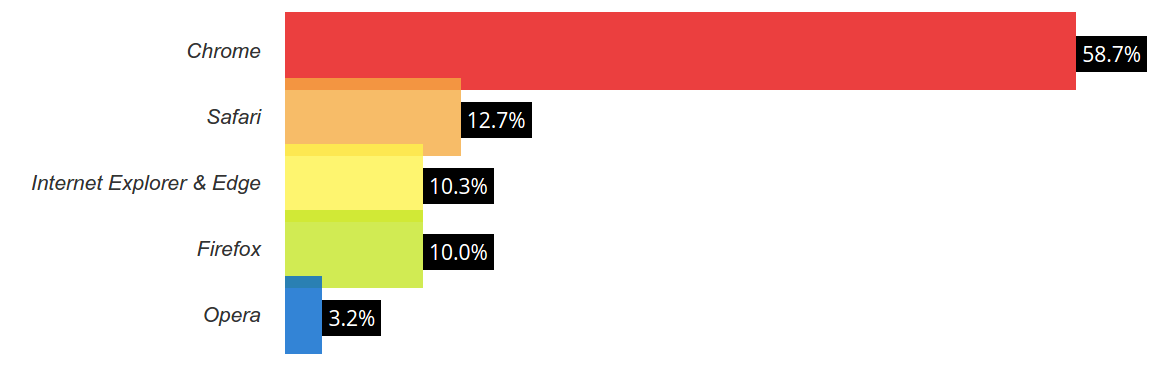
\includegraphics[scale=0.3]{img/browser_2016.png}
  \caption{Die fünf meistgenutzten Browser im Mai 2016 \cite{top-five-browser-statistics}}\label{fig:browser-may-2016}
\end{figure}

\subsection{Interoperabilität}
\label{sec:muster_interoperabilitaet}
Auch bei den Webapplikationen ist es wichtig, bereits existente Frameworks und Problemlösungen nutzen zu können. Folglich müssen externe \ac{JS} und \ac{CSS} Bibliotheken ohne große Probleme eingebettet werden können, ohne den Quellcode zu verändern. Sollte es die Möglichkeit geben bestehende, externe Bibliotheken einzubinden oder anderweitig nutzbar zu machen, gilt das Kriterium als erfüllt.


\subsection{Asynchrone Verarbeitung}
\label{sec:muster_asynchrone_verarbeitung}
Große Datenmengen, deren Übertragung einige Sekunden in Anspruch nimmt, oder Aufgaben die langwierig sind, sollten nicht synchron ausgeführt werden. Stattdessen bietet es sich an, asynchrone Aufgabenblöcke zu definieren, wie beispielsweise das nachladen von Daten, sollten sie tatsächlich angefordert werden. Am Beispiel der hier geplanten \ac{SPA} bedeutet dies, dass Informationen von einem Webserver erst angefordert und sichtbar gemacht werden, sobald der Nutzer diese durch einen Klick auf ein Element anfordert. Da initial gewisse Daten noch nicht vorhanden sind, verringert sich die Datenmenge der zu übertragenen Informationen. Dadurch kann der Webserver entlastet und die initiale Ladezeit der Webseite verringert werden. Um das Kriterium der asynchronen Verarbeitung zu erfüllen, sollte Elm die Möglichkeit liefern, asynchrone Requests an einen Server zu schicken, Daten anzufordern und die Antwort darzustellen, oder andere langwierige Aufgaben asynchron zu verarbeiten. Die Applikation darf dabei nicht in einen undefinierten Zustand kommen, sprich durch beispielsweise eine langsame Übertragungsrate Fehler bei der Darstellung erzeugen oder die Ausführung von nachfolgenden Operationen verzögern.


\subsection{Dateigröße}
\label{sec:muster_dateigroesse}
Die Größe einer Datei wirkt sich auf die Dauer der Übertragungszeit aus. Ist die Datenmenge groß, steigt entsprechend auch die Dateigröße an. Eine schlechte Übertragungsrate kann somit zu erheblichen Verzögerungen der fertigen Darstellung führen. Um die Dateigröße von üblichen \ac{JS}-Dateien zu verringern, werden oftmals externe Tools zur Entfernung von Leerzeichen oder der Verkürzung von Funktions- und Variablennamen genutzt. Für die anschließende Bewertung dieses Kriteriums, sollte der Compiler die Möglichkeit zur automatischen Verkleinerung der Dateigröße mit einer Effizienz von mindestens 50\% bieten. Zusätzlich sollte die Dateigröße eines Elm-Programmes mit den eingebundenen Standard-Bibliotheken $elm-lang/core$ und $elm-lang/html$ die Dateigröße der Frameworks $AngularJs$, $Ember$ und $React$ nicht übersteigen. Die Größen der einzelnen Frameworks werden dabei der Statistik von Anton Vynogradenko, verfügbar unter \url{https://gist.github.com/Restuta/cda69e50a853aa64912d} entnommen. Dabei wird jeweils die neueste Version der Statistik gewählt. Dem zugeordnet werden die Ergebnisse für Elm.

\newpage
\section{Empirische Analyse}
\label{sec:Empirische Analyse}
Die folgende Sektion unterstützt und erläutert die praktische Ausarbeitung der \ac{SPA}. Dabei wird zunächst der typische Programmablauf der Applikation erörtert. Ferner wird die Entwicklungsumgebung unter der die Applikation ausgearbeitet wurde vorgestellt. Die Entwicklung wird in einzelne Abschnitte unterteilt und einzeln erläutert.

\subsection{Programmablauf}
\label{sec:Programmablauf}
Abbildung XY: Zeigt die Kommunikation zwischen Client und Webserver
Die Abbildung XY zeigt die geplante Kommunikation zwischen dem Client und dem Webserver.
In Schritt 1 fordert der Nutzer die Webseite an und erzeugt dadurch einen Request. Dieser geht in Schritt 2 bei dem Webserver ein und wird verarbeitet. Abhängig von der angeforderten URL erzeugt der Webserver eine Antwort, mit allen zu sendenden Informationen und dem dazugehörigen \ac{HTML}, \ac{CSS} und \ac{JS} Code. Im nächsten Schritt 3 werden diese Daten zurück an den Client gesendet. Der Client nimmt die Daten entgegen, wie in Schritt 4 beschrieben. Des Weiteren macht der Client die Daten entsprechend sichtbar, so dass der Nutzer eine vollständige Präsentation der Webseite sieht. Schritt 5 beschreibt die mögliche Interaktion des Nutzers mit dem ihm präsentierten Dokument. Jede Interaktion wird durch \ac{JS} erkannt und erzeugt eine Reaktion. Unter Umständen ist dies ein Request an den Server, womit bei Schritt 1 begonnen wird. Externe Daten wie Stylesheets oder bestehende \ac{JS}-Skripte  werden asynchron nachgeladen, wie es Schritt 6 andeutet. Dabei kann dieser Schritt zeitlich gesehen zu jedem Zeitpunkt nach Schritt 3 geschehen.
%TODO: Abbildung einfügen: Seite 68


\subsection{Entwicklungsumgebung}
\label{sec:Entwicklungsumgebung}
Die zugrunde liegende Elm-Version ist 0.17 und wird unter Ubuntu 14.04 64bit installiert. Als Editor wird Atom mit den Elm-spezifischen Plugins $language-elm$, $linter-elm-make$ und $elm-format$ verwendet. Diese Plugins unterstützen die Entwicklung von Elm-Programmen, indem der Quellcode beim speichern automatisch dem Style-Guide entsprechend formatiert, eventuelle Fehler bei der Kompilierung direkt im Editor sichtbar gemacht und der Code syntaktisch gefärbt, sowie Vorschläge zur Vervollständigung des geschriebenen Quellcodes gemacht werden. Da die Pakete ständig aktualisiert und verändert werden, wird an dieser Stelle von einer detaillierten Beschreibung zur Installation und Verwendung abgesehen und auf die Dokumentationen der einzelnen Pakete verwiesen.
Der angefertigte Quellcode wird durch den Compiler $elm-make$ kompiliert.
Anschließend wird die fertige \ac{SPA} mit den Browsern Google Chrome (Version 51), Internet Explorer (Version XY), Mozilla Firefox (Version 47) und Opera (Version 38). In Bezug auf die Abbildung~\ref{fig:browser-may-2016} fällt auf, dass Safari als einziger der fünf meistgenutzten Browser nicht getestet wird. Zum Zeitpunkt dieser wissenschaftlichen Arbeit stand kein entsprechendes Testgerät zur Verfügung. Die in der Abbildung genannten Browser decken 94,9\% aller genutzten Browser ab. Abzüglich des Browsers Safari, werden entsprechend die verbleibenden 82,2\% aller Browser überprüft.


TODO: (https://github.com/triforkse/atom-elm-format)\\
(https://github.com/triforkse/atom-elm-format)\\
(https://atom.io/packages/language-elm\\

\subsection{Grundaufbau}
\label{sec:Grundaufbau}
Damit der Nutzer letzten Endes eine Webseite besuchen kann, muss zunächst ein auslieferbares Dokument erzeugt werden. Hierfür wird zunächst die $index.html$-Datei aus dem Template $Agency$ übernommen und entsprechend angepasst. Die Datei dient dabei als Grundgerüst für die Elm-Applikation und lädt externe \ac{CSS} und \ac{JS}-Dateien.
Zunächst wird sämtlicher Code Code der für die Darstellung des Templates innerhalb des $body$-Elementes definiert wurde entfernt. Lediglich die $script$-Tags bleiben innerhalb des $body$s bestehen, so dass sämtliche vordefinierte \ac{JS}-Dateien weiterhin geladen werden.
\begin{figure}[p]
\centering
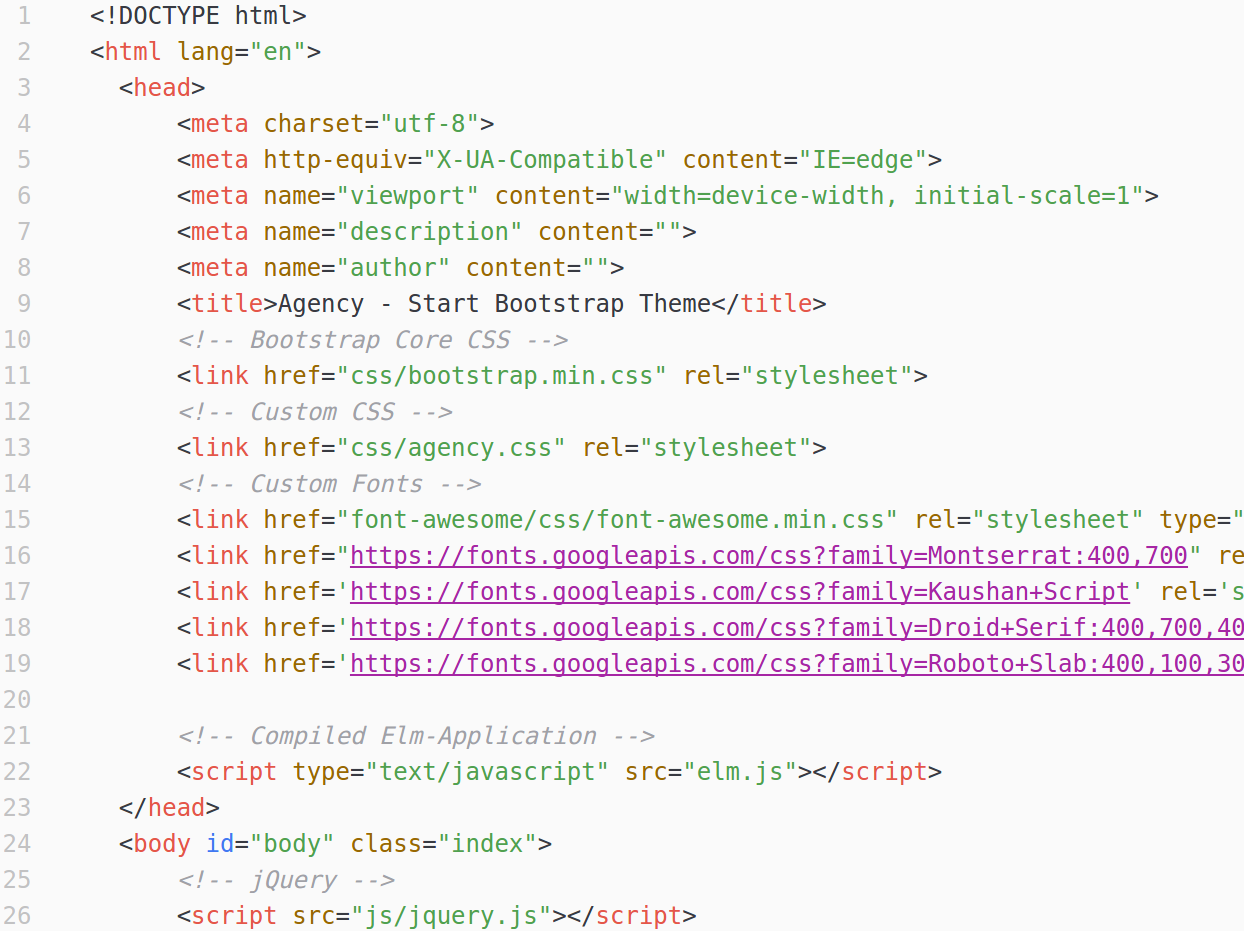
\includegraphics[scale=0.32]{img/index-grundaufbau-1.png}
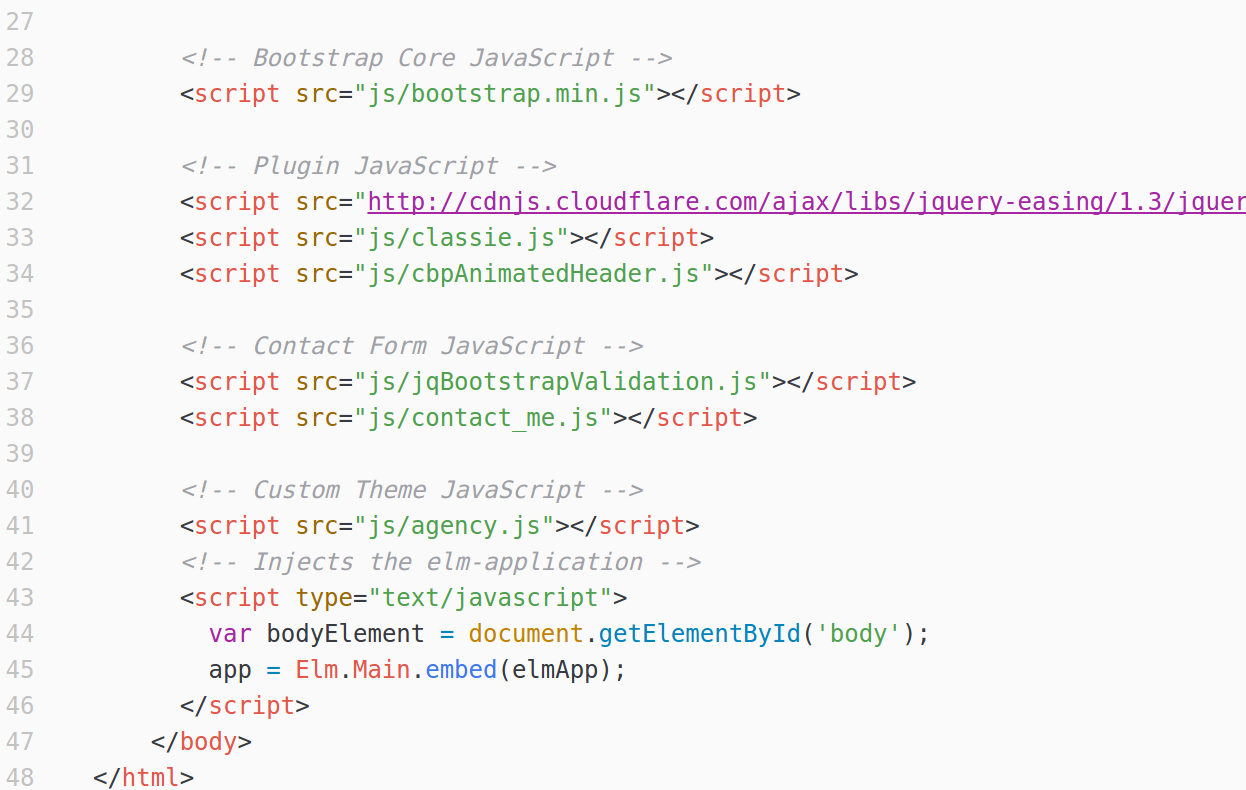
\includegraphics[scale=0.32]{img/index-grundaufbau-2.png}
\caption{Grundaufbau der $index.html$, um die Elm-Applikation zu injizieren}\label{fig:index-grundaufbau}
\end{figure}

\begin{figure}[p]
\centering
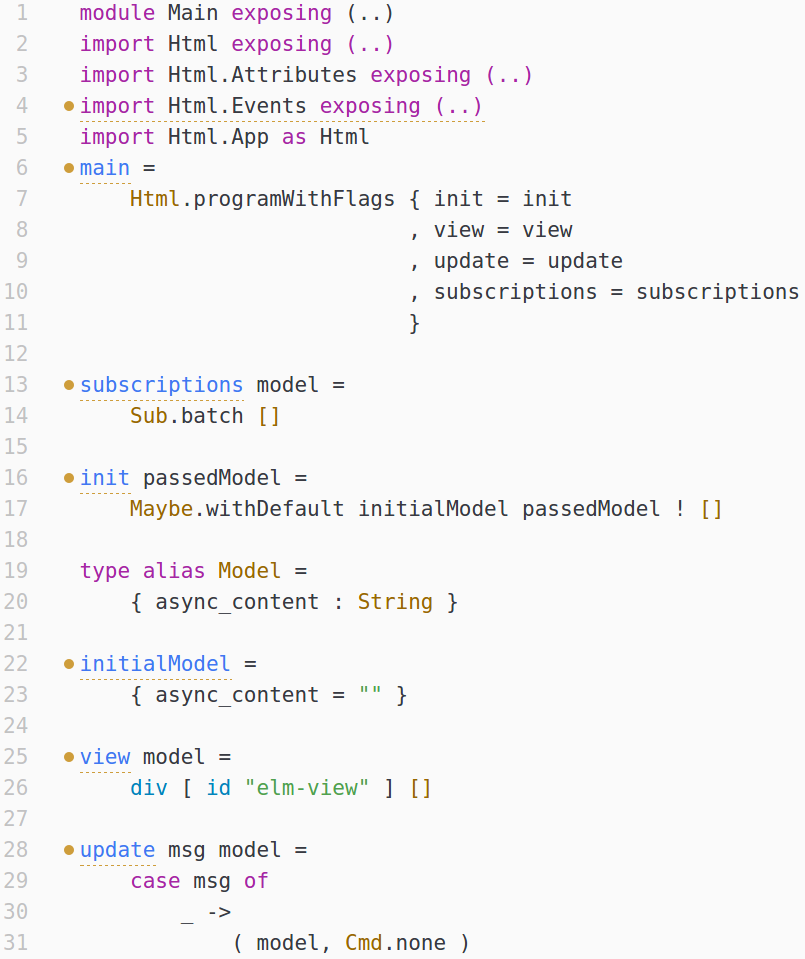
\includegraphics[scale=0.5]{img/elm-grundaufbau-start.png}
\caption{Grundgerüst der Elm-Applikation}\label{fig:elm-grundaufbau-start}
\end{figure}
Damit in das Grundgerüst die Elm-Applikation geladen werden kann, ist ein weiterer $script$-Tag notwendig, der die kompilierte Elm-Applikationsdatei $elm.js$ einbindet. Des Weiteren muss die Elm-Applikation explizit aufgerufen und gestartet werden. Die Abbildung~\ref{fig:index-grundaufbau} zeigt die $index.html$ mit den notwendigen Änderungen in Zeile $22$, in welcher die kompilierte Elm-Applikation eingebunden wird, sowie den Zeilen $43$ bis $46$, in denen die Applikation gestartet wird und ein Ziel-\ac{HTML}-Element übergeben bekommt. Damit die Datei $elm.js$ eingebunden werden kann, muss sie zunächst erstellt werden. Dafür wird der Elm-Compiler $elm-make$ mit dem Zusatz $Main.elm\,--output\,elm.js$ genutzt. Hierbei wird die Datei $Main.elm$ kompiliert und das Ergebnis in die Datei $elm.js$ gespeichert.
Es bestehen insgesamt drei Möglichkeiten die Elm-Applikation innerhalb der $index.html$ aufzurufen:
\begin{enumerate}
\item{$fullscreen$}: Der erzeugte Code der Applikation wird in den $body$-Tag einer \ac{HTML}-Datei geladen und überschreibt den sonstigen \ac{HTML}-Code

\item{$embed$}: Der erzeugte Code der Applikation wird in den übergebenen DOM-Knoten geladen

\item{$worker$}: Initialisiert die Applikation ohne grafische Benutzeroberfläche
\end{enumerate}
Die Abbildung~\ref{fig:index-grundaufbau} zeigt, dass für dieses praktische Beispiel Version $2$ genutzt wird. Diese Version bietet den Vorteil, dass eine Elm-Applikation gezielt in einen vordefinierten Bereich einer gesamten Webseite platziert werden kann. Auf diese Weise kann eine Elm-Applikation problemlos in eine bestehende Webseite eingebaut und erweitert werden. Ferner erlaubt diese Art der Injizierung zusätzliche externe \ac{JS}- und \ac{CSS}-Dateien hinzuzufügen.
Nutzt man beispielsweise Version $1$, so ist die Elm-Applikation im absoluten Vordergrund und lässt die Interaktion mit anderen Elementen die zuvor auf der Webseite definiert wurden nicht mehr zu. Version $3$ wiederum erzeugt keine grafische Benutzeroberfläche, wodurch ebenso keine Interaktion möglich ist.
Wahlweise besteht die Möglichkeit über den mitgelieferten Elm-Webserver $elm-reactor$ die Applikation manuell zu starten. Jedoch wird die Elm-Applikation dabei als $fullscreen$-Applikation gestartet und ist für die Zwecke dieser Arbeit nicht geeignet, weswegen auf die manuell Kompilierung zurückgegriffen werden muss.

Zusätzlich zum Grundgerüst der $index.html$ muss nun noch das Grundgerüst der eigentlichen Elm-Applikation erstellt werden. Wie im Kapitel \nameref{sec:Konzept} beschrieben, ist Elm nach einem Model-View-Update-Konzept aufgebaut. Entsprechend sind das die drei notwendigen Funktionen, die es zu realisieren gilt, damit die Elm-Applikation lauffähig ist. Um \ac{HTML}-Code zu erzeugen gibt es das Elm-Paket $elm-lang/html$. Es liefert einerseits die Funktionen um \ac{HTML}-Elemente zu erzeugen, andererseits drei Funktionen $beginnerProgram$, $program$ und $programWithFlags$. Diese kümmern sich um die Bereitstellung und Auslieferung der Applikation, so dass sich Entwickler ganz auf die eigentliche Programmierung konzentrieren können. Dabei variieren stets die Übergabeparameter, wodurch die Applikation leicht erweitert und komplexer werden kann. So verlangt die Funktion $beginnerProgram$ nur die bekannten Funktionen $model$, $view$ und $update$ als Übergabeparameter. Hierbei können jedoch keine asynchronen Funktionen wie \ac{HTTP}-Requests genutzt werden.
Dafür gibt es wiederum die erweiterte Funktion $program$, die als vierten Übergabeparameter sogenannte $subscriptions$ erwartet. Sie werden für die Kommunikation zwischen Elm und \ac{JS}, sowie Verbindungen zu Websockets genutzt.
Die dritte und letzte Möglichkeit der Initialisierung ist die Funktion $programWithFlags$. Hierbei wird die Übergabe eines initialen $Model$s an die Elm-Applikation ermöglicht, um den Zustand der Applikation dynamisch setzen zu können.
\begin{figure}[ht]
\centering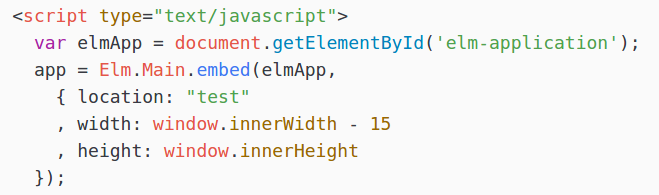
\includegraphics[scale=0.6]{img/programWithFlags_pass_data.png}
\caption{Eine beispielhafte Initialisierung der Elm-Applikation mit initialen, dynamischen Werten}\label{fig:programWithFlags}
\end{figure}
Die Abbildung~\ref{fig:programWithFlags} zeigt beispielhaft die Implementierung der $Html.App.programWithFlags$-Funktion. Der zweite Übergabeparameter an die $Elm.Main.embed$-Funktion ist dabei ein $Record$ mit den gewünschten initialen Werten.
Für die Umsetzung dieses praktischen Beispiels ist der Grundaufbau wie in Abbildung~\ref{fig:elm-grundaufbau-start} notwendig. Dies sind die minimal notwendigen Funktionen, um in den weiteren Schritten die einzelnen Sektionen des Views von \ac{HTML} nach Elm zu portieren, in einzelne Funktionen auszulagern und letzten Endes der Versuch, die gesamte Applikation zu modularisieren.
Aus der Abbildung~\ref{fig:elm-grundaufbau-start} wird ersichtlich, dass zunächst das gesamte Paket $elm-lang/html$ importiert wird. Die vorherige Installation des Pakets ist analog zu der in der Abbildung~\ref{fig:elm-install-package} beschriebene Vorgehensweise. Des Weiteren wird der Grundaufbau der Elm-Applikation ersichtlich.
Innerhalb der $main$-Funktion werden dabei alle notwendigen Funktionen an die $HTML$-Bibliothek weitergereicht. Dazu gehören die $init$, $view$, $update$ und $subscriptions$-Funktionen. Wie der Name bereits suggeriert initiiert die $init$-Funktion ein $Model$. Dabei wird dieses entweder anhand der dynamisch übergebenen Werte, oder durch ein Ausweich-Model ($initialModel$) erstellt, falls keine Daten übergeben wurden.
Die Funktion $view$ erzeugt in der Abbildung~\ref{fig:elm-grundaufbau-start} zunächst ein $div$-Element, während die $update$-Funktion auf jede eingehende Interaktion ein Tupel mit einem unveränderten $model$, sowie keinem $Effekt$ zurück gibt. Um die Applikation aufzurufen muss die Datei $index.html$ im Browser geöffnet werden.


\subsection{Überführung des Views}
\label{sec:ueberfuehrung-view}
Nachdem der Grundaufbau der Elm-Applikation beidseitig ausgeführt wurde, können nun die einzelnen Sektionen der originalen $index.html$ aus dem $Agency$-Template nativ in Elm überführt werden. Dafür wird das Online-Tool $html-to-elm$ auf der Webseite \url{http://mbylstra.github.io/html-to-elm/} zur Hilfe genommen. Der gesamte zuvor im $body$-Tag befindliche \ac{HTML}-Code wird kopiert und zur Konvertierung in das entsprechende Textfeld des Tools eingefügt. Der konvertierte Elm-Code sollte daraufhin auf der gegenüberliegenden Seite zu sehen sein. Durch einen Klick auf $copy$ wird der erstellte Elm-Code in die Zwischenablage kopiert, so dass der Inhalt in die $view$-Funktion der $Main.elm$-Datei eingefügt werden kann. Der kopierte Text fungiert dabei als kompletter Rückgabewert der $view$-Funktion.
\begin{figure}[h]
\centering
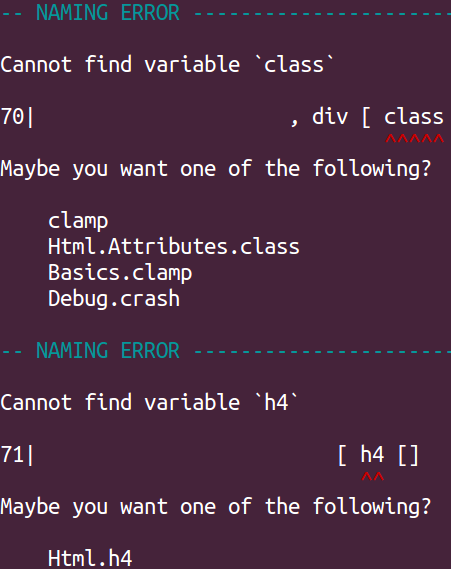
\includegraphics[scale=0.5]{img/elm-naming-error.png}
\caption{Elm-Compilerfehler bei fehlenden Funktionen im Namensraum}\label{fig:elm-naming-error}
\end{figure}
Das Tool $html-to-elm$ sollte den Code bereits nach den Regeln des Style-Guides formatiert haben, so dass hiermit der erste Schritt der Portierung abgeschlossen ist. Um Namenskonflikte im aktuellen Namensraum zwischen Funktionen zu verhindern, werden innerhalb der importierten $HTML$-Bibliothek die genutzten Funktionen zur Erstellung von \ac{HTML}-Code explizit genannt. Der Compiler sollte nach dem Entfernen des Kommandos $exposing (..)$ eine Warnung ausgeben und auf die fehlenden Funktionen hinweisen, wie es in Abbildung~\ref{fig:elm-naming-error} gezeigt wird. Schlägt der Compiler dabei vor, die Funktion aus dem Namensraum $Html.Attributes$ aufzurufen, muss sie entsprechend in die Liste der zu ladenden Funktionen der $Attribute$ hinzugefügt werden, wie in Abbildung~\ref{fig:elm-grundaufbau-start} in Zeile 3. Die Funktionen zur Generierung von \ac{HTML}-Tags hingegen sollten in die Liste der $import\,Html$s stehen. Nachdem alle Funktionen korrekt in den aktuellen Namensraum aufgenommen wurden, sollten keinerlei Compilerfehler auftreten.


\subsection{Beheben von JavaScript-Fehlern}
\label{sec:javascript-errors}
Das Öffnen der Seite mitsamt der Developer-Tools von Google-Chrome verrät, dass die bisher eingebundenen \ac{JS}-Dateien nicht fehlerfrei funktionieren. Nutzt man das Template wie vorgesehen, ist sämtliche Funktionalität vorhanden. Bei der Überführung des Templates in Elm gilt es allerdings zu beachten, dass die Elm-Applikation den $view$ ausliefert und diesen erst verzögert darstellt. Dem menschlichen Betrachter fällt dies zwar nicht auf, jedoch greifen die \ac{JS}-Skripte auf ein noch nicht geladenes Element zu. Es ist dementsprechend notwendig, die einzelnen Skripte anzupassen und mit Hilfe der $\$(document).ready()$-Funktion des Frameworks $jQuery$ (\url{https://learn.jquery.com/using-jquery-core/document-ready/}) erst nach dem kompletten Seitenaufbau zu laden.
Innerhalb der Datei $agency.js$ muss nicht nur die Funktion $\$('a.page-scroll').bind(...)$, sondern auch die nachfolgenden Funktionen innerhalb des $\$(function(){..});$-Blocks liegen. Die \ac{JS}-Datei $cbpAnimatedHeader.js$ hingegen erzeugt einen Fehler, wie in Abbildung~\ref{fig:js-classie-error} zu sehen ist.
\begin{figure}[h]
\centering
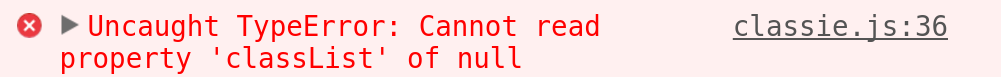
\includegraphics[scale=0.4]{img/error-javascript-classie.png}
\caption{JavaScript-Fehler innerhalb der Developer-Tools}\label{fig:js-classie-error}
\end{figure}
Um diesen zu beheben, muss der gesamte Dateiinhalt in eine $\$(document).ready()$-Funktion geschachtelt werden. Zusätzlich dazu ist es notwendig, dass die Codezeile wie sie in Abbildung~\ref{fig:code-to-add} zu sehen ist, als erstes in der Funktion $scrollPage()$ hinzugefügt wird.
\begin{figure}[h]
\centering
header = document.querySelector( '.navbar-fixed-top' );
\caption{Notwendiger Code, um JavaScript-Fehler zu beheben.}\label{fig:code-to-add}
\end{figure}
Der Code hat zur Folge, dass das Navigations-Element ausgewählt und an die $classie$-Funktion weitergegeben wird. Fehlt diese Zeile, erfolgt ein Aufruf der $classie$-Funktion mit einem undefinierten Wert, wodurch der Fehler in Abbildung~\ref{fig:js-classie-error} zustande kommt. Nachdem diese beiden Fehler behoben wurden, kann nun die $Scroll-Spy$-Funktionalität auf der Webseite betrachtet werden. Scrollt der Nutzer nun auf oder ab und befindet sich dabei in einer innerhalb der Navigation definierten Sektion, so wird das entsprechende Gegenstück in der Navigationsleiste farblich hinterlegt. Des Weiteren verkleinert sich die Navigationsleiste, wenn der Nutzer eine bestimmte Entfernung nach unten gescrollt hat.


\subsection{Auslagern des Views}
\label{sec:auslagern-des-views}
Um die einzelnen Sektionen der Webseite im Quellcode klar voneinander zu trennen, werden die einzelnen Sektionen in eine jeweils eigene Funktion ausgelagert.
Für jede Sektion wird hierfür eine gleichnamige Funktion angelegt, die dem Muster in Abbildung~\ref{fig:elm-view-section} folgt. Die $id$ eines \ac{HTML}-Elementes könnte entsprechend für den Funktionsnamen $nameDerSektion$ genutzt werden, da dieses Attribut ohnehin einzigartig in einem gesamten \ac{HTML}-Dokument vorkommt und eine klare Namensgebung liefert.
\begin{figure}[htb]
\centering
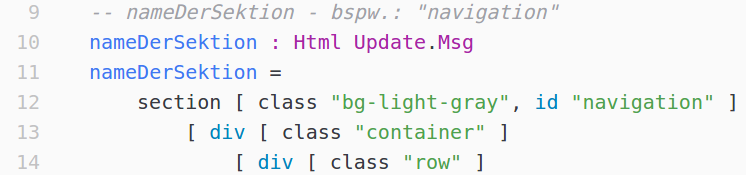
\includegraphics[scale=0.53]{img/elm-html-sections.png}
\caption{Deklaration einer Sektion des Views in Elm}\label{fig:elm-view-section}
\end{figure}
Am Beispiel der $portfolio$-Sektion des zu überführenden Templates sehen die daraus resultierende Funktion teilweise aus wie in Abbildung~\ref{fig:elm-view-section-function}. Die einzelnen Klassen und ID`s wurden beibehalten und übernommen. Nachdem die einzelnen Sektionen in Funktionen ausgelagert wurden fällt auf, dass die Sektionen nicht mehr angezeigt werden. Dafür ist es notwendig die ursprüngliche $view$-Funktion mit den Funktionsaufrufen der Sektionen zu versehen. Dieses Vorgehen kann in der Abbildung ~\ref{fig:elm-view-sections-call} betrachtet werden. Das Resultat der $view$-Funktion ist unverändert, ist jedoch nun im Code übersichtlicher.
\begin{figure}[h]
\centering
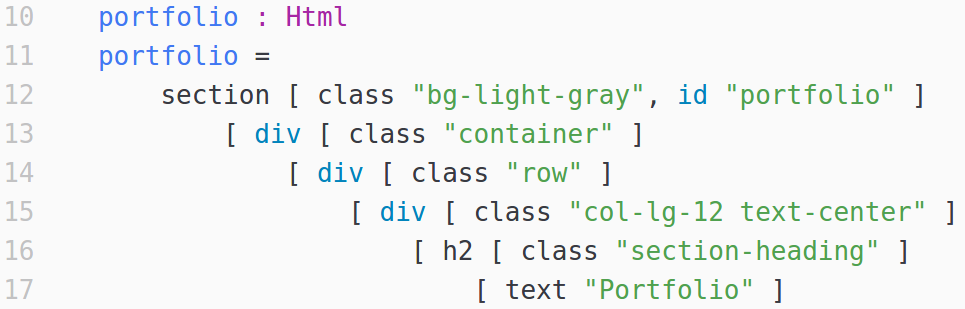
\includegraphics[scale=0.41]{img/elm-view-portfolio-section-function.png}
\caption{Ausgelagerter View in eine eigene Funktion}\label{fig:elm-view-section-function}
\end{figure}

\begin{figure}[h]
\centering
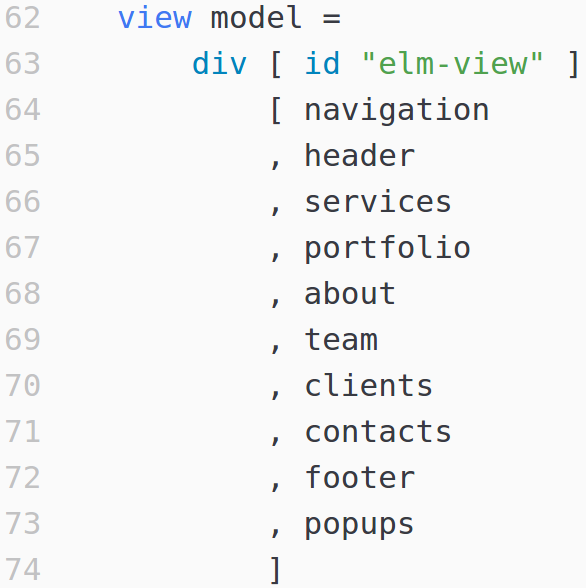
\includegraphics[scale=0.4]{img/elm-view-section-functions-calling.png}
\caption{Aufruf der einzelnen Sektionen im View}\label{fig:elm-view-sections-call}
\end{figure}


\subsection{Hinzufügen von Klick-Events}
\label{sec:erweiterung-clicks}
Der derzeitige Stand der überführten Applikation stellt bereits sämtliche Sektionen auf der Webseite dar und erlaubt das Öffnen eines Modals durch einen Klick auf eines der Portfolio-Elemente. Bei einem Klick auf ein Element in der Navigationsleiste springt der Viewport des Browsers jedoch ohne jegliche Verzögerung direkt auf die ausgewählte Sektion. Das ursprüngliche Template hingegen nutzt die Funktionalität $smooth-page-scrolling$, wodurch der Nutzer einen sichtbaren Scroll-Effekt erhält, während automatisch zur ausgewählten Sektion gescrollt wird. Innerhalb der Datei $agency.js$, in der vorab bereits die Funktion des $Scroll-Spy$s wiederhergestellt wurde, wird in den Zeilen $9$ bis $15$ die Funktionalität des automatischen scrollens bei einem Klick umgesetzt, wie in Abbildung~\ref{fig:non-functional-scrolling} zu sehen ist.
\begin{figure}[h]
\centering
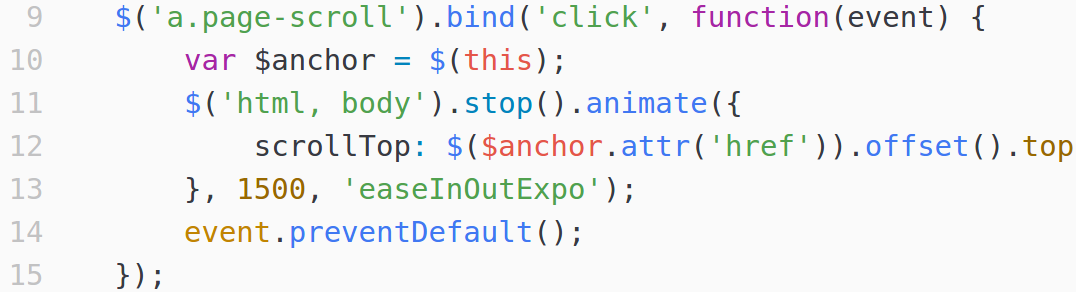
\includegraphics[scale=0.37]{img/non-functional-scrolling}
\caption{Funktion zum scrollen bei einem Klick}\label{fig:non-functional-scrolling}
\end{figure}
Dabei wird zunächst ein $Ereignisbehandler$ an die Link-Elemente mit der Klasse $page-scroll$ gebunden. Klickt der Nutzer eines dieser Elemente, so wird die darauf folgende Funktion ausgeführt. Diese Funktion wiederum ließt Informationen des angeklickten Elementes aus, insbesondere das $href$-Attribut, welches die Id zur angeklickten Sektion enthält. Mittels der $animate$-Funktion wird letztlich zur gewünschten Sektion gescrollt.
Diese Funktionalität ist nicht verfügbar, da das externe \ac{JS} versucht auf \ac{HTML}-Elemente innerhalb der Elm-Applikation zuzugreifen. Um dieses Problem zu lösen, kann einerseits die Funktion innerhalb der Datei $agency.js$ umgeschrieben werden, so dass sämtliche Klicks innerhalb des $body$-Elementes abgefangen werden, da sich dieser nicht Teil der Elm-Applikation ist. Andererseits kann der Klick innerhalb der Elm-Applikation registiert und über sogenannte Ports nach außen getragen werden. In diesem Beispiel ist das die bevorzugte Methode, da so eine klare Trennung zwischen der Elm-Applikation und den externen \ac{JS}-Skripten herrscht.
Die Elm-Bibliothek $Html.Events$ enthält die Methode $onWithOptions$, mit Hilfe derer ein Klick auf ein Element des $views$ in Elm eine $Msg$ erzeugt. Diese $Msg$ wird an die $update$-Funktion weitergeleitet und kann dort entsprechend ausgewertet werden.
\begin{figure}[htb]
\centering
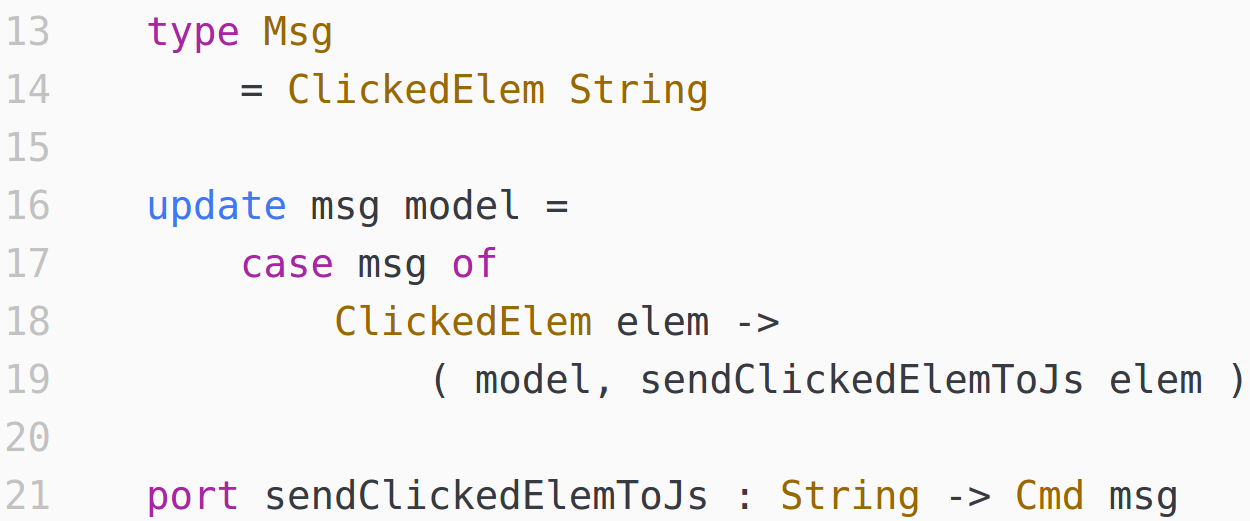
\includegraphics[scale=0.3]{img/elm-port.png}
\caption{Definition eines neuen Union Types, sowie eines Ports für die Kommunikation zwischen Elm und \ac{JS}}\label{fig:create-port}
\end{figure}
Bislang gibt es in der Elm-Applikation noch keine $Msg$-Typen, welche die $update$-Funktion verarbeiten könnte. Dementsprechend wird zunächst ein neuer Union-Type $Msg$ mit dem Eintrag $ClickedElem\,String$ angelegt. Der Union-Type muss nun noch in der $update$-Funktion behandelt werden. Hierbei wird ein neuer $case$ angelegt, mit dem zuvor erstellten Eintrag $ClickedElem$ und dem Übergabeparameter $elem$ vom Typ $String$. Der vorherige Eintrag "$\_ ->$", welcher für alle Fälle gilt, kann entfernt werden. Der Rückgabewert des $ClickedElem$-Falles ist dabei ein Tupel, bestehend aus dem unveränderten $model$, sowie einem Effekt. In diesem Fall ist der Effekt das Senden der ausgewählten Elemente nach außen zu einem \ac{JS}-Skript, das die Daten verarbeitet. Der Effekt wird dabei über den Port $sendClickedElemToJs$ nach außen geschickt. Der Port muss definiert werden mit dem Kommando in Zeile $21$ aus der Abbildung~\ref{fig:create-port}. Das Kommando ist lediglich die Signatur der gewünschten Kommunikationsweise und wird durch den Elm-Compiler während des Kompiliervorgangs entsprechend verarbeitet.
Beim Versuch den Code wie er in Abbildung~\ref{fig:create-port} zu sehen ist zu kompilieren, wird der Compiler mit der Fehlermeldung "You are declaring port $sendClickedElemToJs$ in a normal module" antworten. Die Fehlermeldung bedeutet, dass das Modul in dem ein Port definiert wird explizit als ein Port-Modul deklariert werden muss. Die erste Zeile des Hauptmoduls muss folglich noch mit dem Schlüsselwort $port$ versehen werden. Damit die Elm-Applikation die Funktion $ClickElem$ aufruft, bedarf es noch des Aufrufes der zuvor erwähnten $onWithOptions$-Methode. Diese wird in den $view$ an den entsprechenden Stellen eingesetzt. Die Links der Navigationsleiste befinden sich in der Funktion $navigation$ und müssen um den Zusatz der $onWithOptions$-Funktion, sowie den Übergabeparametern $ClickedElem$ und dem $href$-Wert erweitert werden. In Abbildung~\ref{fig:elm-view-onclick} kann beispielhaft die Erweiterung an einigen Stellen begutachtet werden. Die Funktion $onWithOptions$ bekommt dabei zunächst einmal das $Event$, auf das sie einen Ereignishandler setzen soll. In diesem Fall ist dies ein $click$. Darauf folgt ein optionaler $Record$ von Typ $Options$. Hier müssen die Werte $stopPropagation$ und $preventDefault$ auf $True$ gesetzt werden. Fehlt diese Einstellung, so wird das scrollen sofort ausgeführt und kann möglicherweise andere Ergebnisbehandler in denen der Link geschachtelt ist ausführen. Dies würde zu einem undefinierten Verhalten führen. Der letzte Parameter ist die die Decoder-Funktion $Json.succeed$. Sie führt dazu, dass die übergebene Funktion $ClickedElem$ direkt und ohne weitere Überprüfungen ausgeführt wird.
\begin{figure}[hbt]
\centering
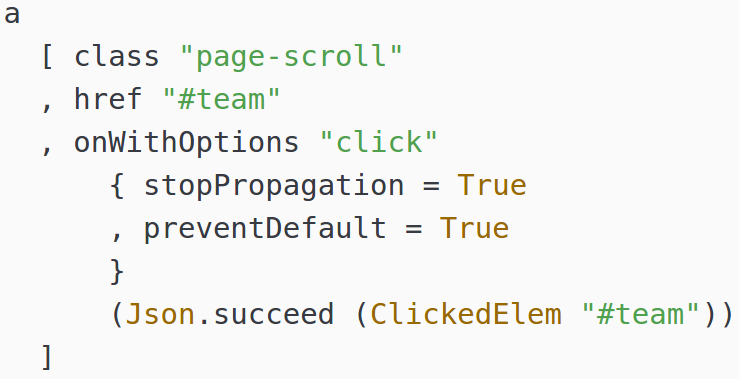
\includegraphics[scale=0.4]{img/elm-view-onclick.png}
\caption{Erweiterung des Views um einen $onWithOptions$ Ereignisbehandler in Elm}\label{fig:elm-view-onclick}
\end{figure}
Seitens der Elm-Applikation ist die notwendige Erweiterung nun abgeschlossen. Jedoch muss noch die $index.html$ um eine sogenannte $subscription$ erweitert werden. Das bedeutet, dass innerhalb der $index$-Datei die Nachricht der Elm-Applikation des angeklickten Elements entgegengenommen und verarbeitet werden muss. Diesbezüglich wird in der $index.html$ nach der Codestelle die für die Initialisierung der Elm-Applikation zuständig ist die Funktion aus Abbildung~\ref{fig:scrollTop} hinzugefügt.
\begin{figure}[hbt]
\centering
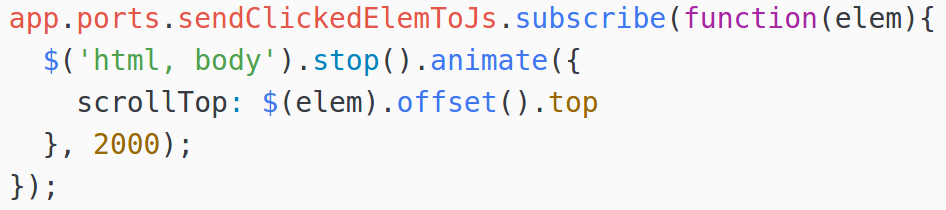
\includegraphics[scale=0.4]{img/scrollTop.png}
\caption{Entgegennahme der Daten aus der Elm-Applikation und anschließendes scrollen}\label{fig:scrollTop}
\end{figure}
Durch das Kommando $app.ports.sendClickedElemToJs.subscribe$ werden sämtliche Daten die Elm über den Port $sendClickedElemToJs$ sendet entgegengenommen und die nachfolgende Funktion ausgeführt. Diese Funktion wurde in diesem Beispiel lediglich aus der Datei $agency.js$ kopiert. Sie ermittelt das \ac{HTML}-Element im Baum anhand der übergebenen Id und scrollt innerhalb von zwei Sekunden zur obersten Stelle des übergebenen Elements.

\subsection{Modularisierung der Applikation}
\label{sec:modularisierung-der-applikation}
Durch das Auslagern aller einzelnen Sektionen der darzustellenden \ac{HTML}-Elemente ist die daraus resultierende $Main.elm$-Datei recht unübersichtlich. Abhängigkeiten zwischen einzelnen Funktionen sind kaum mehr erkennbar und die Programmlogik ist nicht unterscheidbar von Funktionen, die für die Darstellung des Views zuständlich sind. Folglich ist es sinnvoll einzelne Teile der Applikation in mehrere Dateien und Ordner zu verschieben. Eine solche Strukturierung hilft dabei, die womöglich fehlerbehafteten Teile der Applikation schneller zu finden und die einzelnen Bereiche der Applikation deutlicher voneinander zu trennen. Dabei werden die einzelnen Programmteile des Views ausgelagert in eigene Module. Dasselbe Prinzip wird für das Model und die Update-Funktion angewandt. Im Gegenzug sollen die ausgelagerten Programmteile global im Hauptmodul importiert und an den entsprechenden Stellen aufgerufen werden.

\subsubsection{View}
\label{sec:auslagern-view}
Jede Funktion die bisher eine Sektion des Views erzeugt hat, wird in eine neu angelegte $.elm$-Datei verschoben und die Funktion umbenannt zu $view$. Die Datei bekommt dabei den Namen, den die Funktion vorher trug. Ferner wird ein Ordner $View$ erzeugt, in den all diese Dateien hin verschoben werden. Damit die neuen Dateien als Module eingebunden werden können, müssen sie als solches definiert werden. Das bedeutet, dass jede Datei mit dem Kommando $module\,View.NameDerDatei\,exposing\,(view)$ initialisiert werden muss. Der Zusatz $view$ nach dem Kommando $exposing$ gibt an, dass die Funktion $view$ nach außen hin sichtbar ist und vom importierenden Modul genutzt werden kann.
\begin{figure}[hbt]
\centering
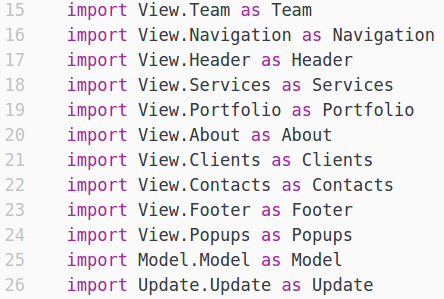
\includegraphics[scale=0.5]{img/imports-main.png}
\caption{Einbindung und Aufruf der ausgelagerten View-Funktionen}\label{fig:elm-main-view-imports}
\end{figure}
Nachdem alle Funktionen in ein eigenes Modul ausgelagert wurden, müssen alle Module im Hauptmodul $Main.elm$ importiert werden. Des Weiteren müssen die $view$-Funktionen der einzelnen Module im Hauptmodul aufgerufen werden. Die Abbildungen~\ref{fig:elm-main-view} und \ref{fig:elm-main-view-imports} zeigen die $view$-Funktion des Hauptmoduls, sowie den Aufruf um die angelegten Module zu importieren.
\begin{figure}[hbt]
\centering
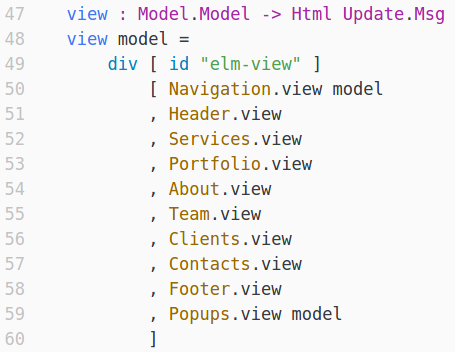
\includegraphics[scale=0.6]{img/view-main.png}
\caption{Einbindung und Aufruf der ausgelagerten View-Funktionen}\label{fig:elm-main-view}
\end{figure}
Letzten Endes müssen die einzelnen Module noch mit den notwendigen $import$s für die verwendeten Funktionen erweitert werden. Das Hauptmodul wiederum kann von den nicht benutzten $Html$- beziehungsweise $Html.Attributes$-Funktionen gesäubert werden.

\subsubsection{Update}
\label{sec:auslagern-update}
Nicht nur die für die Darstellung verantwortlichen Funktionen sollten modularisiert werden, sondern auch die Programmlogik. Hierfür wird ein weiterer Ordner $Update$ erzeugt. Die bisherige $update$-Funktion wird demzufolge analog zu den $View$-Funktionen ausgelagert in ein eigenes Modul im neu erzeugten Ordner $Update$. Das $Update$-Modul folgt derselben Namensgebung wie ein einzelner $View$ und wird definiert als $Update.Update$. Zusätzlich müssen auch an dieser Stelle die $import$s der benutzten Pakete übernommen und definiert werden, wobei das Hauptmodul diese entfernen kann.

\subsubsection{Model}
\label{sec:auslagern-Model}
Letztlich wird noch das $model$, das sämtliche Daten die den Status der Applikation beschreiben enthält, in ein eigenes Modul im Unterordner $Model$ überführt. Die Einbindung dieses Moduls funktioniert analog zur Modularisierung von $Update$ und $View$.
Mit Hilfe dieser Modularisierung wird das angestrebte \ac{MVU}-Konzept von Elm besonders deutlich.


\subsection{Asynchrones Laden von Daten}
\label{sec:async-laden}
Klickt man innerhalb der Portfolio-Sektion der Webseite auf ein Element, öffnet sich ein Modal in dem weitere Informationen dargestellt werden. Die bestehende Elm-Applikation wird nun um das Feature des asynchronen Ladens von Informationen erweitert, die anschließend in dem geöffneten Modal angezeigt werden. Beispielhaft wird hier die \ac{API} von \ac{ICNDb} (\url{https://api.icndb.com}) genutzt. Sie liefert bei jeder Anfrage einen zufälligen Witz zurück.
Für dieses Funktionalität muss zunächst das $model$ erweitert und angepasst werden, da dies die einzige Möglichkeit in einer Elm-Applikation ist, Daten beziehungsweise den Status der Applikation zu speichern. Das $model$ bekommt entsprechend ein weiteres Feld $async\_content$ vom Typ $String$.
Bei einem Klick auf einen der Portfoliobeiträge soll ein Modal geöffnet und ein zufälliger Witz präsentiert werden. Dafür wird über die externe \ac{API} ein zufälliger String angefordert, vom Server generiert und letztlich an die Elm-Applikation zurückgegeben. Ebenso wäre es möglich einen Server für das Backend zu erstellen, auf dem eine Datenbank läuft, so dass Daten asynchron angefordert werden können. Das asynchrone Anfordern von Daten basiert sowohl bei einem lokalen, wie auch externen Server auf dem gleichen Konzept, weswegen dieser Schritt entfällt und der vorhandene externe Service genutzt wird.
Ein solcher asynchroner Request stellt im Grunde eine Verletzung des Konzeptes von Elm dar, dass es keinerlei Seiteneffekte gibt. Da nicht bekannt ist, wann der Request endet und welchen Status die Antwort besitzt, ist zunächst nicht vorhersehbar, wie der Status der Applikation nach dem Request aussehen wird. Um dieses Problem zu vermeiden, ist es notwendig alle möglichen Fälle, sprich den Fall einer erfolgreichen, sowie fehlerhaften Übertragung, zu behandeln. Auf diese Weise ist gewährleistet, dass die Applikation sich nicht plötzlich in einem undefinierten Zustand befindet. Es bedarf zusätzlich der Bibliotheken $Http$, $Json.Decode$ und $Task$, damit ein asynchroner Request ausgeführt werden kann. Die Bibliotheken müssen installiert und in die jeweiligen Module importiert werden. Des Weiteren gilt es den Klick auf den Portfoliobeitrag abzufangen, um den Request zu starten und das Ergebnis in den View einzuarbeiten. Dafür gibt es die $onClick$ Funktion aus der $Html.Events$-Bibliothek. Sie bekommt eine auszuführende Funktion aus dem $Update$-Modul als Parameter, in diesem Fall $GetRandomString$, wie es in Abbildung~\ref{fig:portfolio-async} zu sehen ist. Bei einem Klick auf das Element wird eine $Msg$ von diesem Typ erstellt und muss in der $update$-Funktion behandelt werden.
\begin{figure}[h]
\centering
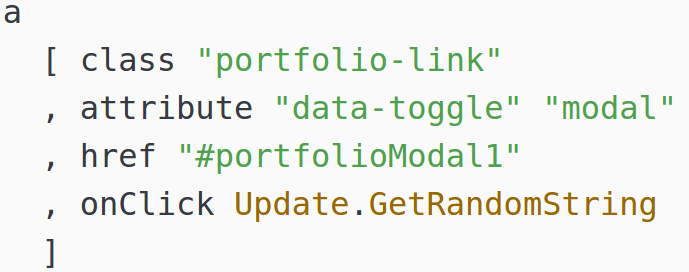
\includegraphics[scale=0.4]{img/portfolio-async.png}
\caption{OnClick-Ereignisbehandler in Elm}\label{fig:portfolio-async}
\end{figure}
Wie zuvor bei der Definition einer $Msg$ um Daten durch Ports nach außen zu kommunizieren, muss auch die Nachricht $GetRandomString$ als $Msg$-Typ deklariert werden, um so in der $update$-Funktion behandelt werden zu können. Außerdem müssen die möglichen Statusfälle des Requests behandelt und als $Msg$ hinzugefügt werden. Abbildung~\ref{fig:msg-async} zeigt die hinzugefügten $Msg$-Typen.
\begin{figure}[h]
\centering
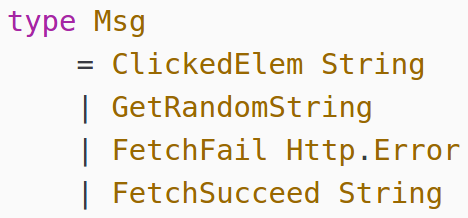
\includegraphics[scale=0.5]{img/msg-async.png}
\caption{$Msg$-Deklaration mit asynchronem Request}\label{fig:msg-async}
\end{figure}
Nachdem die neuen Interaktionsmöglichkeiten in der Elm-Applikation implementiert wurden, muss nun der eigentliche Request ausführbar gemacht werden. Die Funktion $GetRandomString$ soll dabei ein unverändertes Model, sowie eine asynchron auszuführende Funktion in Form eines Effektes als Tupel zurückliefern. Dabei ist die asynchrone Funktion der eigentliche \ac{HTTP}-Request, wie er in Abbildung~\ref{fig:fetchasync-async} erkennbar ist.
\begin{figure}[h]
\centering
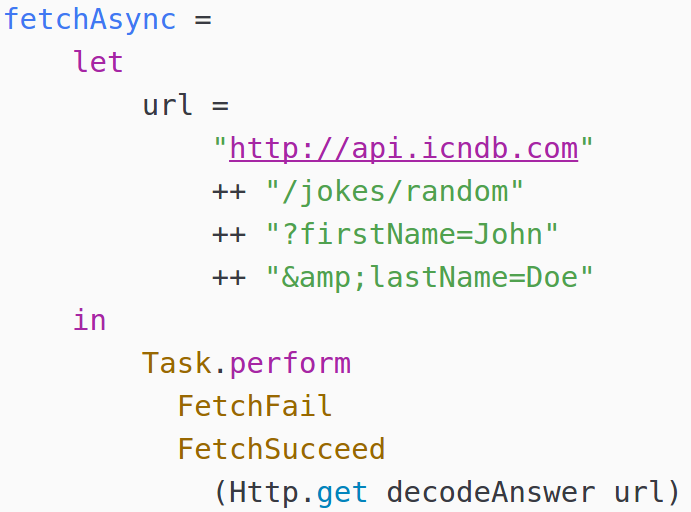
\includegraphics[scale=0.3]{img/fetchasync-async.png}
\caption{Asynchroner \ac{HTTP}-Request in Elm}\label{fig:fetchasync-async}
\end{figure}
Dabei wird die Funktion $Http.get$ genutzt, um einen Request an die $url$ auszuführen. Die Antwort des Requests wird an die Funktion $decodeAnswer$ gereicht, welche das eingehende \ac{JSON}-Objekt dekodiert und die gewünschten Informationen herausfiltert. Die Dekodierfunktion kann in Abbildung~\ref{fig:decodeanswer-async} betrachtet werden. Sie filtert das geschachtelte \ac{JSON}-Objekt, so dass nur der gewünschte String übrig bleibt.
\begin{figure}[h]
\centering
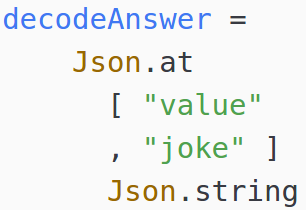
\includegraphics[scale=0.4]{img/decodeanswer-async.png}
\caption{Dekodierung eines Json-Objektes in Elm}\label{fig:decodeanswer-async}
\end{figure}
Abhängig vom Status des Requests, wird der jeweilige Fall in der $update$-Funktion aufgerufen. Bei einer erfolgreichen Übertragung wird die Funktion $FetchSucceed$ ein neues Model mit dem asynchron abgerufenen String zurückliefern. Der String wird dabei in das Feld $async\_content$ des $model$ geschrieben. Bei einer fehlgeschlagenen Übertragung wird die Funktion $FetchFail$ das unveränderte $model$ zurückgeben. Alternativ kann auch eine mögliche Fehlermeldung in das $model$ eingearbeitet und im $view$ dargestellt werden.
\begin{figure}[h]
\centering
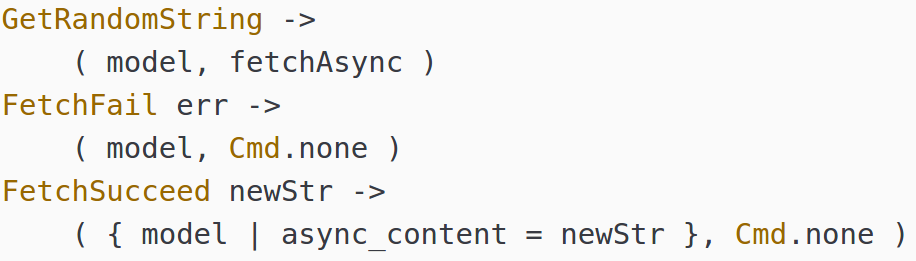
\includegraphics[scale=0.4]{img/update-async.png}
\caption{$Update$-Fälle für den asynchronen Request}\label{fig:update-async}
\end{figure}
Die fertige $update$-Funktion mit allen abgehandelten Fällen ist in Abbildung~\ref{fig:update-async} dargestellt. Der asynchrone Request wird dabei durch $GetRandomString$ initiiert. Die Manipulation des $model$ findet lediglich in der $FetchSucceed$-Funktion statt.
Nachdem die Elm-Applikation an dieser Stelle fehlerfrei kompiliert wurde, kann der asynchrone Request auf der Webseite getestet werden. Mit Hilfe der Developer-Tools kann die ausgehende Anfrage an den \ac{ICNDb}-Server beobachtet und ausgewertet werden. Auch die Antwort des Servers kann unbehandelt in Abbildung~\ref{fig:request-async} begutachtet werden.
\begin{figure}[htb]
\centering
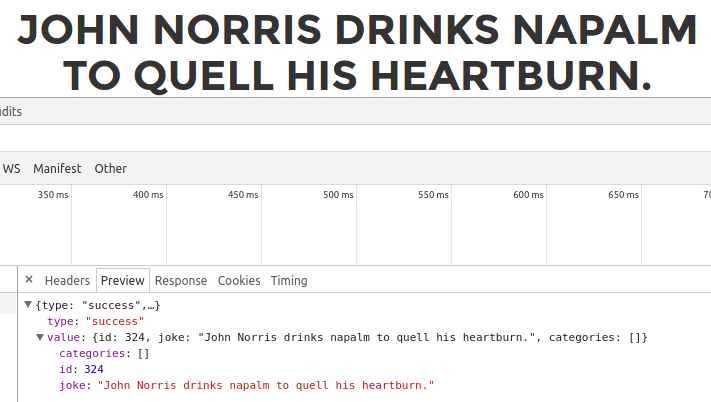
\includegraphics[scale=0.4]{img/request-async.png}
\caption{Ausgehender HTTP-Request und eingehende Antwort}\label{fig:request-async}
\end{figure}
Die Abbildung zeigt ferner wie der zurückgelieferte Text des Requests fehlerfrei dekodiert und in das $model$ übertragen, sowie letztlich in der $view$-Funktion des $Popup$-Moduls mittels des Kommandos $text\,model.async\_content$ angezeigt wird.



\subsection{Beobachtungen}
\label{sec:Beobachtungen}
In diesem Abschnitt sollen Auffälligkeiten, die während der Überführung des $agency$-Templates in eine native Elm-Applikation auftraten, aufgezeigt und erläutert werden. Es handelt sich hierbei nicht nur um Probleme, sondern auch um interessante Erkenntnisse im Hinblick auf die Unterschiede zwischen herkömmlicher Webentwicklung mit \ac{HTML}, \ac{CSS} und \ac{JS} gegenüber Elm, die es zu erwähnen gilt.

\subsubsection{Natives Einbinden von CSS in Elm nur beschränkt möglich}
Herkömmlicherweise können Elemente einer \ac{HTML}-Datei auf drei Arten gestylt werden.
\begin{enumerate}
\item{Inline \ac{CSS}:}
	\subitem Das Inline \ac{CSS} erlaubt Design-Anpassungen für genau ein bestimmtes Element. Der verfasste \ac{CSS}-Code kann nicht von anderen Elementen genutzt werden und wird über das \ac{HTML}-Attribut $style$ eingeführt.
\item{Internes \ac{CSS}:}
	\subitem \ac{HTML} enthält den $style$-Tag. In diesem kann natives \ac{CSS} verfasst, bestimmte Klassen oder Id's erstellt und sämtliche gängigen Design-Anpassungen durchgeführt werden.
\item{Externes \ac{CSS}:}
	\subitem Die Erweiterung des internen \ac{CSS} ist das externe \ac{CSS}, bei dem der gesamte \ac{CSS}-Code ausgelagert wird in eine eigene $.css$-Datei. Diese wird wiederum mit Hilfe des $link$-Tag der \ac{HTML}-Datei eingebunden.
\end{enumerate}
In Elm ist es nicht möglich nativen \ac{CSS}-Code zu verfassen. Jedoch kann mittels der Bibliothek $elm-lang/html$ inline \ac{CSS} erzeugt werden. Das Design wird dabei nativ in Elm über die $Html.style$-Funktion programmiert. Ferner ist das erstellen von $style$-Tags in Elm nicht möglich, wodurch auch die Möglichkeit für internes \ac{CSS} entfällt. Es ist zwar praktisch möglich externe \ac{CSS}-Dateien in die Elm-Applikation nativ in Elm einzubinden, jedoch stört das immens die Nutzbarkeit der Applikation. Die Elm-Applikation wird zunächst ohne das \ac{CSS} geladen, während die externe Datei nachgeladen wird. Das bedeutet für den Nutzer der Webseite, dass zunächst nur Texte und Bilder ohne Styling angezeigt werden. Nachdem die externe Datei vollständig übertragen wurde, wird das darin enthaltene Design auf die \ac{HTML}-Elemente angewandt. Der zeitliche Abstand zwischen initialem Laden und der Anwendung des Stylesheets hat ein sichtbares $flackern$ zur Folge, wodurch eine Nutzung in einem fertigen System entfällt. Dies ist der Grund, weswegen bereits bestehende \ac{CSS}-Dateien des Templates nicht nativ in Elm überführt, sondern über das \ac{HTML}-Grundgerüst eingebunden wurden. Zusätzlich zu diesem Umstand wird inline- und internes \ac{CSS} nicht vom Browser zwischengespeichert. Das hat eine längere Ladezeit zur Folge und sollte vermieden werden. Des Weiteren ist es nur bedingt möglich \ac{CSS}-Code in Elm an mehreren Stellen zu verwenden, wie es üblicherweise mit in \ac{CSS} definierten Klassen der Fall ist.


\subsubsection{HTML-Code ist in Elm wesentlich kürzer}
\ac{HTML}-Tags mit den gleichnamigen Funktionen nativ in Elm zu erstellen ist einerseits signifikant kürzer, andererseits viel übersichtlicher als das Verfassen von herkömmlichen \ac{HTML}-Code.
\begin{figure}[h]
\centering
HTML:
<div>
</div>\\
Elm:
div[$\,$][$\,$]
\caption{Ein $div$-Element in \ac{HTML} und Elm}\label{fig:div-element}
\end{figure}
Die Abbildung~\ref{fig:div-element} zeigt ein $div$-Element, wie es einerseits in klassischem \ac{HTML}, andererseits in Elm realisiert wird. In Elm handelt es sich dabei um einen Funktionsaufruf mit zwei Parametern, in diesem Fall zwei leeren Listen. Ein \ac{HTML}-Element hat dabei eine Anzahl von $5+2*n_0$ Zeichen, wobei $n_0$ gleich der Zeichenanzahl des Tag-Namens und $5$ die Zeichen für das öffnende, sowie schließende Tag sind. Am Beispiel des $div$-Elementes wäre $n_0:=3$, wodurch die Implementierung in \ac{HTML} $5+2*3$, sprich $11$ Zeichen benötigt.
In Elm hingegen benötigt die Erstellung eines \ac{HTML}-Elementes $4+n_1$ Zeichen, wobei $n_1$ gleich der Zeichenanzahl des Tags, sprich hier der Funktion $div$, und $4$ die Zeichenanzahl für die Parameterliste ist. Am selben Beispiel wären das $4+3$, sprich $7$ Zeichen. Die Konstanten $5$ (\ac{HTML}) und $4$ (Elm) können vernachlässigt werden, wodurch sich die dynamischen Werte $2*n_0$ und $n_1$ gegenüberstehen. Da alle \ac{HTML}-Tags in Elm mit einer gleichnamigen Funktion erstellt werden, kann $n_0$ gleich $n_1$ gestellt werden. Daraus folgt, dass Elm im Vergleich zu \ac{HTML} 50\% weniger Zeichen für die Erstellung eines \ac{HTML}-Elementes benötigt.
Die Differenz der Zeichen lässt sich auf das schließen der Tags in \ac{HTML} zurückführen. Nativer Elm-Code arbeitet mit Einrückungen, wohingegen klassischer \ac{HTML}-Code über die öffnenden und schließenden Tags geschachtelt wird. Dadurch entsteht bei \ac{HTML}-Code der Vorteil, dass ein gesamtes Dokument theoretisch in nur einer Zeile ohne Absätze definiert werden kann, während in Elm die Einrückungen und die damit verbundenen Zeilenumbrüche notwendig sind. Daraus folgt, dass Elm-Code zwangsweise übersichtlicher bleibt, da die Einrückungen nicht umgangen werden können und dem Entwickler eine visuelle Rückmeldung liefern. Der Elm-Compiler wird den Elm-Code nicht in \ac{JS}-Code umwandeln, sollten die Abstände inkorrekt sein. \ac{HTML}-Code bietet die Möglichkeit gleichermaßen übersichtlich zu programmieren, jedoch gibt es hier keinen Compiler oder sonstige Warnhinweise für den Fall, dass geschriebener Code unübersichtlich wird.
Durch die Einrückung in das damit verbundene Fehlen von schließenden Tags kam es zu weniger Flüchtigkeitsfehlern in Form von falschen Verschachtelungen oder dem simplen Fehlen der schließenden Tags bei einer tiefen oder über mehrere Absätze stattfindende Schachtelung.

\subsubsection{Elm hat eine stark wachsende Open-Source Gemeinschaft}
Trotzdem Elm erst im März 2012 entwickelt wurde, gibt es bereits eine Vielzahl an Gemeinschaften, um über die Sprache zu diskutieren, Hilfe zu erbitten oder gemeinsam an Projekten zu arbeiten. Neben einem eigenen Slack-Chatroom mit 2.701 angemeldeten Nutzern \cite[vgl.]{slack-user}, gibt es noch die offizielle Google-Gruppe. Offiziell gibt es derzeit $205$ Elm-Bibiliotheken \cite[vgl.]{elm-package}, von denen jede einzelne ein Open-Source-Projekt darstellt und für alle Entwickler freigegeben ist. Auf der Webseite \url{https://github.com/} gibt es zur Zeit 2.845 öffentliche Projekte \cite[vgl.]{elm-repositories} die komplett oder zumindest teilweise in Elm realisiert wurden. Ferner wurden 6.365 Probleme in diesen Projekten gemeldet, von denen 4.834 bereits gelöst und 1.531 noch geöffnet sind.  Alles in Allem wird deutlich, dass Elm eine wachsende Anhängerschaft besitzt und die Probleme der Webentwicklung auf eine andere Weise angeht. Wann immer Fragen auftraten konnten die Nutzer in einer der genannten Medien meist in wenigen Minuten aushelfen. Des Weiteren ist Elm anwendbar auf allen Betriebssystemen, die den \ac{NPM} unterstützen. Zusätzlich gibt es die öffentlichen Tools $elm-repl$, $elm-make$ und $elm-package$, mit denen eine Elm-Applikation umgesetzt werden kann. Darüber hinaus gibt es Quellen wie \url{http://guide.elm-lang.org/}, \url{http://elm-lang.org/get-started} und \url{http://www.elm-tutorial.org/en}, die mit Hilfe von Schritt-für-Schritt Anleitungen und praktischen Beispielen an die Programmiersprache heranführen.


\subsection{Auswertung}
\label{sec:Auswertung}
Nachdem die \ac{SPA} vollständig überführt und einige Beobachtungen erläutert wurden, steht die Auswertung der einzelnen Bewertungskriterien aus. Dieser Abschnitt erläutert dabei in welchem Maße die Kriterien erfüllt wurden und inwiefern die Erkenntnisse verallgemeinerbar sind und auf andere Webapplikationen zutreffen.
\begin{figure}[htb]
\centering
\begin{tabular}{ | p{8cm} | c | }
	\hline
	\textbf{Kriterium} & \textbf{Erfüllt}\\
	\hline
	\ref{sec:muster_wartbarkeit_und_lesbarkeit} \nameref{sec:muster_wartbarkeit_und_lesbarkeit} & \checkmark\\
	\hline
	\ref{sec:muster_zuverlaessigkeit} \nameref{sec:muster_zuverlaessigkeit} & \checkmark\\
	\hline
	\ref{sec:muster_portabilitaet} \nameref{sec:muster_portabilitaet} & \checkmark\\
	\hline
	\ref{sec:muster_effizienz} \nameref{sec:muster_effizienz} & \checkmark\\
	\hline
	\ref{sec:muster_wiederverwendbarkeit} \nameref{sec:muster_wiederverwendbarkeit} & \checkmark\\
	\hline
	\multicolumn{2}{|l|}{\textbf{Webspezifische Kriterien:}} \\
	\hline
	\ref{sec:muster_browser_kompatibilitaet} \nameref{sec:muster_browser_kompatibilitaet} & \checkmark\\
	\hline
	\ref{sec:muster_interoperabilitaet} \nameref{sec:muster_interoperabilitaet} & teilweise erfüllt\\
	\hline
	\ref{sec:muster_asynchrone_verarbeitung} \nameref{sec:muster_asynchrone_verarbeitung} & \checkmark\\
	\hline
	\ref{sec:muster_dateigroesse} \nameref{sec:muster_dateigroesse} & teilweise erfüllt\\
	\hline
\end{tabular}
\caption{Auswertung der Versuchskriterien}
\label{fig:Auswertungstabelle}
\end{figure}

\subsubsection{Auswertung: \ref{sec:muster_wartbarkeit_und_lesbarkeit} \nameref{sec:muster_wartbarkeit_und_lesbarkeit}}
Die Programmiersprache Elm lässt die Erstellung von manuellen Kommentaren zu. Die Kommentare können sich dabei über mehrere Zeilen erstrecken, oder lediglich eine einzige Zeile einnehmen. Für die jeweilige Distanz eines Kommentar gibt es gesonderte Kommandos. Das Atom-Plugin $elm-format$ fügt außerdem Zeilenabstände vor, sowie hinter dem Kommentar ein, so dass es übersichtlich platziert wird. Die Grundlagen dieses Kriteriums wurden somit an dieser Stelle erfüllt. Das fortgeschrittene Kriterium der automatischen Erstellung von Kommentaren mit Informationen über beispielsweise die erwarteten Typen der Übergabeparameter einer Funktion sind nur bedingt erfüllt. Die Möglichkeit $Signaturen$ innerhalb der Elm-Applikation hinzuzufügen besteht und wird durch den $elm-compiler$ unterstützt, allerdings nicht komplett automatisiert. Der Compiler gibt einen Signaturvorschlag in Form einer Warnung ab, sobald die Applikation kompiliert wird, wie es in Abbildung~\ref{fig:compiler-signature-suggestion} demonstriert wird.
\begin{figure}[h]
\centering
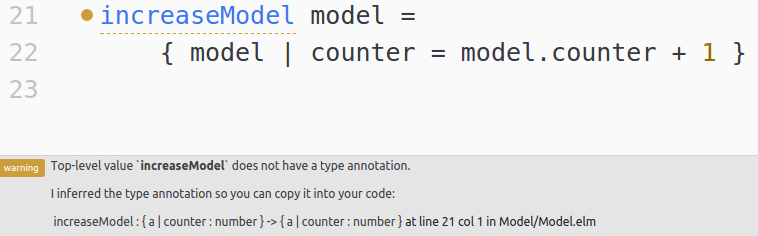
\includegraphics[scale=0.52]{img/compiler_sig_suggestion.png}
\caption{Automatisierter Signaturvorschlag durch den $elm-compiler$}\label{fig:compiler-signature-suggestion}
\end{figure}
Dem Signaturvorschlag kann unter der Prämisse übernommen werden, dass sämtliche zuvor definierten Typen korrekt sind, da der $elm-compiler$ die Vorschläge auf der vorherigen Analyse des gesamten Dokumentes stützt.

\subsubsection{Auswertung: \ref{sec:muster_zuverlaessigkeit} \nameref{sec:muster_zuverlaessigkeit}}
Um die Zuverlässigkeit des $Elm-Compiler$ und die Fehlermeldungen bewerten zu können, werden syntaktische und semantische Fehler innerhalb der Applikation eingebaut. Daraufhin wird eine erwartete Fehlermeldung der tatsächlichen Fehlermeldung gegenübergestellt und die Qualität bewertet.

\textbf{1. Entfernen eines importieren Moduls}\\
\begin{figure}[h!]
\centering
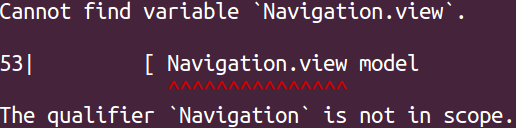
\includegraphics[scale=0.5]{img/import-error.png}
\end{figure}
Die Fehlermeldung des 1. Versuches sagt aus, dass die Variable $Navigation.view$ nicht gefunden wurde und das Modul $Navigation$ nicht im aktuellen Namensraum vertreten ist. Ein Entwickler kann daraus schließen, dass das Modul nicht ordnungsgemäß eingebunden wurde, oder im Namensraum anders benannt wurde. In beiden Fällen wird der Entwickler die importierende Programmstelle aufsuchen, die sich am Beginn der Datei befindet. Die Fehlermeldung gibt einen hilfreichen Aufschluss über das eigentliche Problem.


\textbf{2. Falsche Benennung eines Feldes}\\
\begin{figure}[h!]
\centering
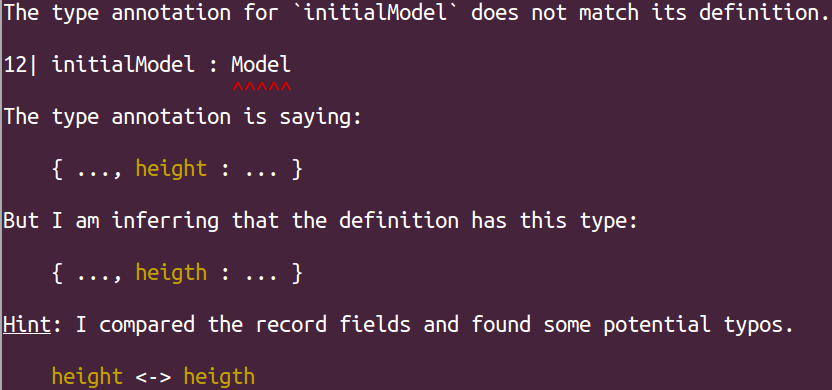
\includegraphics[scale=0.4]{img/definition-error.png}
\end{figure}
Im 2. Versuch wird durch die Fehlermeldung vermittelt, dass das $Model$ per Definition ein Feld mit dem Namen $height$ hat. Im weiteren Verlauf der Applikation hingegen wird ebenfalls auf ein $Model$ zugegriffen, diesmal jedoch auf das Feld mit dem Namen $heigth$. Es handelt sich offensichtlich um einen Schreibfehler. Bei der herkömmlichen Entwicklung mit \ac{JS} ist es möglich, dynamisch Felder in einem Objekt hinzuzufügen, wodurch selbst bei einer expliziten Überprüfung des Quellcodes der Fehler erst während der Laufzeit auftreten würde. Die Fehlermeldung weißt hier explizit auf das Problem hin und veranschaulicht es.

\textbf{3. Falsche Typzuweisung eines Feldes}\\
\begin{figure}[h!]
\centering
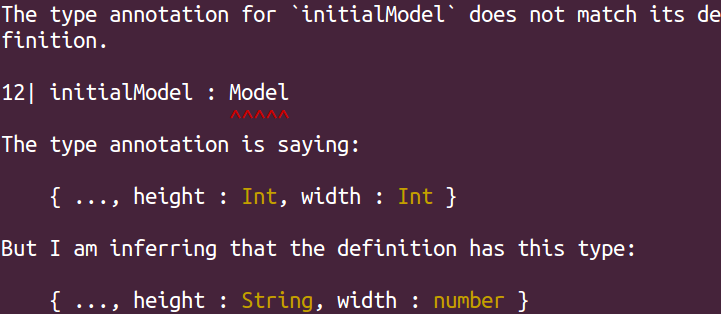
\includegraphics[scale=0.5]{img/types-error.png}
\end{figure}
In der 3. Fehlermeldung wird durch den Compiler erkannt, dass ein Typenfehler aufgetreten ist. Es ist versucht worden das Feld $height$ mit dem Wert $"0"$ zu initialisieren. Lauf Definition ist das Feld allerdings von Typ $Int$, wohingegen versucht wird einen $String$ zuzuordnen. Da Elm statisch typisiert ist, können Variablen nur einen Datentyp annehmen. \ac{JS} liefert die Möglichkeit eine Variable dynamisch zu typisieren. Der Entwickler wird durch die Fehlermeldung explizit auf den entstandenen Fehler hingewiesen.

\textbf{4. Einbau redundanter Kontrollen}\\
\begin{figure}[h!]
\centering
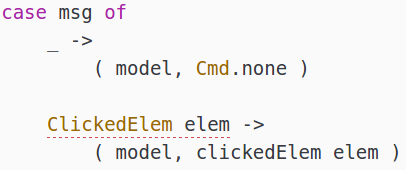
\includegraphics[scale=0.5]{img/redundant-pattern-code.png}
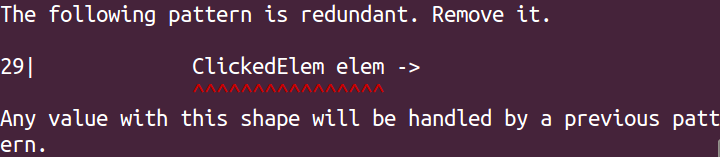
\includegraphics[scale=0.5]{img/redundant-pattern-error.png}
\end{figure}
Für die Demonstration der 4. Fehlermeldung wird einer Kontrollstruktur ein allumfassender Fall hinzugefügt. Der erste Fall der Konstrollstruktur in der Abbildung~\ref{fig:redundant-pattern} ist für jeden zu überprüfenden Fall gültig. Dementsprechend sind alle nachfolgenden Fälle überflüssig, da sie nie erreicht werden können. Der allumfassende Fall kann mit einem $if(true)$-Statement verglichen werden. Jeglicher $else$-Fall in einem solchen Konstrukt wird unmöglich eintreffen. Der $elm-compiler$ erkennt diese Redundanz und gibt an, dass die Fälle bereits behandelt werden und entfernt werden sollten. Dadurch wird zusätzlich die Lesbarkeit des Quellcodes gewahrt, da der Entwickler aufgefordert wird unnötige Codeteile zu entfernen. Erneut gibt die Fehlermeldung ganz klar an, welche Schritte notwendig sind um den Fehler zu beheben.

\textbf{5. Entfernen einer schließenden Klammer}\\
\begin{figure}[h!]
\centering
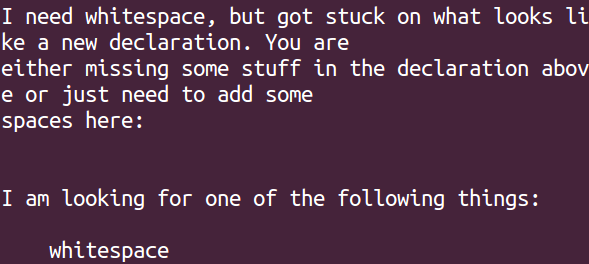
\includegraphics[scale=0.5]{img/missing-brackets-error.png}
\end{figure}
Der 5. Versuch zeigt die Fehlermeldung nachdem eine schließende Klammer eines Statements entfernt wurde. Die daraus resultierende Fehlermeldung gibt an, dass entweder Teile innerhalb der Deklaration fehlen, oder Leerzeichen hinzugefügt werden müssen, um die passende Einrückung zu erreichen. Offensichtlich $fehlt$ etwas in der Deklaration, die Fehlermeldung sollte jedoch wesentlich genauer ausfallen und auf die fehlende Klammer hindeuten. Der Entwickler muss nun die dazugehörige Stelle des Quellcodes absuchen, ohne genau zu wissen, welche möglichen Zeichen fehlen. Diese Fehlermeldung ist nicht ausreichend explizit, um den Fehler ohne Probleme ausfindig zu machen.

\textbf{6. Mehrfache Definition einer Funktion}\\
\begin{figure}[h!]
\centering
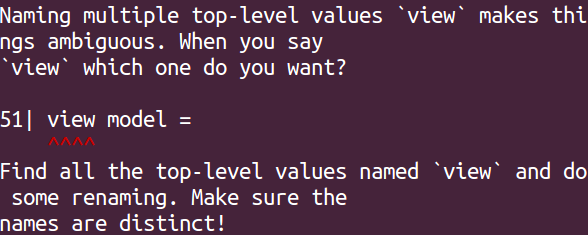
\includegraphics[scale=0.5]{img/multiple-function-definitions.png}
\end{figure}
Die 6. Fehlermeldung bezieht sich auf die mehrmalige Deklaration einer Funktion. Der $elm-compiler$ erkennt, dass mehrere Funktionen mit demselben Namen existieren und sich im gleichen Namensraum befinden. Der Entwickler wird durch die Fehlermeldung dazu aufgefordert, die Funktionen einzigartig zu benennen. Durch die Fehlermeldung erhält der Entwickler eine klare Problemlösung präsentiert.

Die erzeugten Fehler decken offensichtlich nicht alle möglichen Fehlerfälle ab, geben jedoch recht gut Aufschluss über das Verhalten des $elm-compiler$ hinsichtlich gängiger Fehler. Zusammenfassend lässt sich sagen, dass die Fehlermeldungen des $elm-compiler$ zuverlässig Fehler finden, selbst wenn sie über die syntaktische Ebene hinausgehen und den Entwickler über unnötige Kontrollstrukturen informieren. Ferner wird die Qualität der Fehlermeldungen durch das Markieren der tatsächlichen Fehlerposition und dem Unterstreichen der Fehlerquelle verbessert.
Da alle eingebauten Fehler gefunden und die dazugehörigen Fehlermeldungen im Durchschnitt sehr akkurat auf den Fehler hingewiesen haben, kann das Kriterium der Zuverlässigkeit als erfüllt angesehen werden.


\subsubsection{Auswertung: \ref{sec:muster_portabilitaet} \nameref{sec:muster_portabilitaet}}
Die offizielle Webseite von Elm bietet Installationsdateien und -anleitungen für die gängigen Betriebssysteme $Mac$ und $Windows$, sowie für alle Plattformen die den \ac{NPM} unterstützen. Testweise wurde die Elm-Version der \ac{SPA} unter Ubuntu 14.04 64bit, Windows 7 64bit und Windows 10 64bit kompiliert und auf Warnungen oder Fehler seitens des $elm-compiler$ überprüft. In keinem der Fälle kam es zu Fehlern, geschweige denn Warnungen. Das Verhalten des Compilers war unter allen Betriebssystemen gleich und erzeugte keinerlei Anomalien. Das Betriebssystem $Mac$ konnte nicht getestet werden, da zum Zeitpunkt der Auswertung kein passendes Endgerät zur Verfügung stand. Da sowohl $Mac$, als auch $Linux$ auf dem Betriebssystem $Unix$ basieren \cite{http://www.itwissen.info/definition/lexikon/UNIX.html}, wird an dieser Stelle davon ausgegangen, dass der Kompiliervorgang auch unter $Mac$ ohne signifikante Probleme ausführbar ist. Die Abbildung~\ref{fig:elm-compile} zeigt den fehlerfreien Kompiliervorgang der \ac{SPA} unter Ubuntu 14.04 64bit mit Elm 0.17.
\begin{figure}[h]
\centering
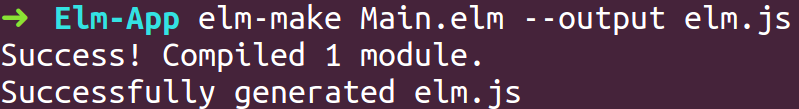
\includegraphics[scale=0.5]{img/elm-compile.png}
\caption{Fehlerfreier Kompiliervorgang durch den Elm-Compiler}\label{fig:elm-compile}
\end{figure}
Das Kriterium der Zuverlässigkeit gilt somit als vollständig erfüllt.


\subsubsection{Auswertung: \ref{sec:muster_effizienz} \nameref{sec:muster_effizienz}}
Innerhalb der Abbildung~\ref{fig:compiler-times} können die Zeiten für die Kompilierung der Elm-Applikation betrachtet werden. Dabei wurde die Dauer des Kompiliervorganges mit und ohne Caching gemessen. Es wurden jeweils zehn Messwerte ermittelt, der jeweils höchste und niedrigste Wert gestrichen und das arithmetische Mittel der verbleibenden acht Werte berechnet. Das Streichen des höchsten und niedrigsten Wert soll etwaigen Messfehlern entgegenwirken. Im Durchschnitt benötigt es 8.03 Sekunden, um die Applikation von Grund auf zu kompilieren. Erlaubt man das Caching der vorherigen Kompiliervorgänge, so ist der erste Durchgang mit 7.88 Sekunden vergleichsweise hoch. Die folgenden Durchgänge hingegen benötigen im Durchschnitt 0.3 Sekunden, unter der Berücksichtigung, dass auch hier der höchste und niedrigste Wert vernachlässigt wird. Dadurch fällt der initial aufwendigste Kompiliervorgang weg. Unter realen Umständen wird ein Entwickler die Applikation unter der Verwendung von Caching kompilieren, womit nur sehr wenig Zeit verloren geht. Ferner kann der Entwickler auf den mitgelieferten Webserver $elm-reactor$ zurückgreifen, der ebenfalls die Applikation bei jedem Seitenaufruf, jedoch nur die tatsächlichen Änderungen neu kompiliert. In beiden Fällen sind die Werte von 8.03 beziehungsweise 0.3 Sekunden für das Kompilieren mehr als annehmbar, insbesondere da ein Entwickler standardmäßig das Caching nutzt. Die Effizienz wird als erfüllt angesehen.
\begin{figure}[h]
\centering
\begin{tabular}{ | c | c | c |}
	\hline
	 \textbf{Durchlauf} 				& \textbf{Dauer ohne Caching} 	& \textbf{Dauer mit Caching}\\
	 \hline
	 1 & 7,56s & \st{7,88s} \\
	 \hline
	 2 & 8,31s & 0,34s\\
	 \hline
	 3 & 7,78s & 0,34s\\
	 \hline
	 4 & 7,77s & 0,31s\\
	 \hline
	 5 & \st{7,4s }& 0,22s\\
	 \hline
	 6 & 8,48s & 0,28s\\
	 \hline
	 7 & \st{9,79s} & \st{0,19s}\\
	 \hline
	 8 & 9,19s & 0,30s\\
	 \hline
	 9 & 6,98s & 0,33s\\
	 \hline
	 10 & 8,14s & 0,28s\\
	 \hhline{|=|=|=|}
	 \textbf{Durchschnitt:} & \textbf{8,03s} & \textbf{0,3s}\\
	 \hline
\end{tabular}
\caption{Zeitliche Auswertung des Kompiliervorganges in Elm}\label{fig:compiler-times}
\end{figure}
Die Performanz der Programmiersprache Elm wird mittels der Applikation $TodoMVC\,Performance\,Comparison$ ausgewertet. Die Applikation liefert Ergebnisse für die Benchmark-Tests der Programmiersprachen Backbone 1.1.2, Ember 1.4.0 mit Handlebars 1.30, Angular 1.2.14, React 0.10.0, Om 0.5.0 mit React 0.9.0, Mercury 3.1.7 mit virtual-dom 0.8, sowie Elm 0.12.3 mit virtual-dom 0.8. Dabei nutzen die Programmiersprachen Elm, Om und Mercury das Konzept der $virtual-dom$.
\begin{figure}[ht]
\centering
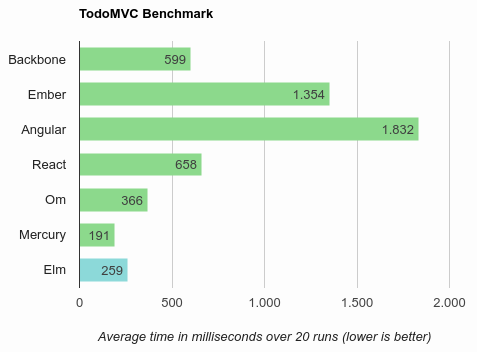
\includegraphics[scale=0.6]{img/elm-benchmark-final.png}
\caption{Benchmark der TodoMVC in unterschiedlichen Programmiersprachen}\label{fig:elm-todo-benchmarks}
\end{figure}
Die zu testenden Programmiersprachen sind weit verbreitet in der Webentwicklung. Die Abbildung~\ref{fig:elm-todo-benchmarks} zeigt eine graphische Auswertung nach 20 ausgeführten Tests. Bei jedem Testdurchlauf wird dabei die Zeit gemessen, die für die Erstellung von 100 Elementen, dem Anklicken all dieser erstellten Elemente sowie dem Löschen aller Elemente benötigt wird. Der Test wurde auf dem in der Sektion~\ref{sec:Entwicklungsumgebung} beschriebenem System ausgeführt. Abbildung~\ref{fig:elm-todo-benchmarks} zeigt, dass Elm durchschnittlich 259ms für einen Test benötigt hat. Den niedrigsten Wert mit 191ms pro Durchlauf erzielte Mercury und ist damit mehr als ein viertel mal schneller als Elm. Den schlechtesten Wert erzielte das Framework AngularJs mit 1832ms pro Durchlauf. Dieser Wert schneidet mehr als 6x schlechter ab, als es bei Elm der Fall war.
Obwohl die gegenübergestellten Programmiersprachen in der Testumgebung nicht den neuesten Versionen entsprechen, ist davon auszugehen, dass die grobe Platzierung selbst mit den neuesten Versionen ähnlich ausfällt. Die einzelnen Frameworks haben an der grundlegenden Umsetzung zur Darstellung von Daten im Browser nichts geändert, das bedeutet, dass Elm, Mercury und Om weiterhin mit neueren Versionen der $virtual-dom$ arbeiten. Die Frameworks Angular, Backbone und Ember nutzen noch immer nicht standardmäßig das Konzept der $virtual-dom$. Lediglich das Framework React könnte bei einem Test der neuesten Version signifikante Veränderung aufweisen, da hier ein $virtual-dom$ Konzept implementiert wurde.
Das Kriterium der Performanz einer Elm-Applikation gilt als erfüllt. Im Vergleich zu anderen beliebten Frameworks schlägt sich Elm mit Bravour und wird nur von $Mercury$, einem extrem leichtgewichtigem Framework übertrumpft.

\subsubsection{Auswertung: \ref{sec:muster_wiederverwendbarkeit} \nameref{sec:muster_wiederverwendbarkeit}}
Das Konzept der Wiederverwendbarkeit, insbesondere der Modularität wird in Elm komplett durchgesetzt. Jede Datei in Elm ist zwangsläufig ein Modul, insofern man die darin enthaltenen Funktionen nutzen möchte. Zusätzlich ist auch ein Zugriffsschutz gegeben. Das bedeutet, dass Funktionen gesondert nach außen hin sichtbar und somit nutzbar gemacht werden können. Gängige imperative Programmiersprachen wie beispielsweise $C++$ nutzen Klassen anstelle von Modulen. Dabei wird der Zugriff von außen auf eine Funktion innerhalb der Klasse durch die Schlüsselwörter $public$, $private$ und $protected$ definiert. Jedes Schlüsselwort bietet einen sichereren Zugriffsschutz. Ähnlich fungiert in Elm das Schlüsselwort $exposing$, wodurch einzelne Funktionen an die importierenden Module zugreifbar gemacht werden. Der Entwickler hat dadurch die Sicherheit, dass nur die von ihm erwarteten Funktionen, sprich die \ac{API}, genutzt werden. Dementsprechend ist das Bewertungskriterium der Wiederverwendbarkeit in allen Aspekten erfüllt.


\subsubsection{Auswertung: \ref{sec:muster_browser_kompatibilitaet} \nameref{sec:muster_browser_kompatibilitaet}}
Wie in Sektion~\ref{sec:Entwicklungsumgebung} angesprochen, werden lediglich die Browser Google Chrome (Version 51), Internet Explorer (Version XY), Mozilla Firefox (Version 47) und Opera (Version 38) getestet. Dabei wird in jedem Browser die $index.html$ der \ac{SPA} aufgerufen und gewartet, bis die Seite komplett geladen ist. Anschließend werden die $onClick$-Elemente der Applikation getestet, indem auf die einzelnen Reiter in der Navigation geklickt wird. Die Webseite soll daraufhin zu den entsprechenden Stellen im Dokument scrollen und die Navigationsleiste kleiner werden. Sobald die $Portfolio$-Sektion erreicht wurde, wird das erste Element angeklickt und überprüft, ob ein asynchroner Request erzeugt, sowie die Ergebnisse in das geöffnete $Modal$ eingepflanzt wurden.

Die Darstellung in allen Browsern ist komplett gleich. Es gibt nur marginale Unterschiede in der Darstellung der \ac{SPA} selbst, die jedoch auf die Unterschiede der Browser selbst zurückzuführen sind. Zusätzlich erzeugt der Aufruf und die Interaktion mit der Webseite in keinem getesteten Browser einen Fehler. Ferner funktioniert die asynchrone Verarbeitung nach einem Klick auf eines der Portfolio-Elemente problemlos und zügig. Auch die Darstellung des Modals unterscheidet sich nicht. Alles in Allem scheint sich die kompilierte Elm-Applikation in allen getesteten Browsern gleich zu verhalten. Das Kriterium der Browser-Kompatibilität gilt als komplett erfüllt.

\subsubsection{Auswertung: \ref{sec:muster_interoperabilitaet} \nameref{sec:muster_interoperabilitaet}}
Das Einbinden von externen \ac{JS}-Frameworks oder bestehendem \ac{CSS}-Code ist nicht vollständig in Elm gegeben. Die Programmiersprache Elm liefert mehrere Möglichkeiten eine Elm-Applikation im Browser darzustellen. Die Methoden dafür können bei Bedarf in der Sektion~\nameref{sec:Grundaufbau} nachgelesen werden. Abhängig von der Art der Initialisierung der Elm-Applikation entsteht eine Abhängigkeit zu einer $.html$-Datei, in welcher der Grundaufbau der Webseite erstellt und die Elm-Applikation geladen wird. Nutzt man eine $.html$-Datei und lädt dort die Elm-Applikation hinein, können bestehende \ac{CSS}- oder \ac{JS}-Frameworks innerhalb des $head$-Tag in einem $link$- oder $script$-Tag geladen werden. Hier entstehen keinerlei Probleme. Wird allerdings die Abhängigkeit der $.html$-Datei umgangen, wird die Elm-Applikation entweder im Vollbildmodus, oder im Hintergrund gestartet und muss somit zwangsweise das Einbinden externer Quellen übernehmen. Diese Funktionalität ist gegeben, jedoch sehr umständlich und nicht nutzbar für ein fertiges Produkt. Beim Einbinden von externem \ac{CSS} durch nativen Elm-Code wird ein $link$-Tag innerhalb des $body$-Tags erstellt und der Inhalt asynchron nachgeladen. Üblicherweise wird externer \ac{CSS}-Code innerhalb des $head$-Tags geladen und auf das gesamte Dokument angewandt. Insofern wäre es nicht problematisch, jedoch bewirkt das Einbinden des Stylings innerhalb des $body$-Tags ein flickern, wodurch zunächst der gesamte Inhalt des Dokumentes komplett ohne und kurze Zeit später mit dem definierten \ac{CSS}-Code angezeigt wird. Des Weiteren bietet die $elm-lang/html$-Bibliothek keine native Funktion für einen $script$ oder $link$-Tag. Stattdessen muss die $Html.node$-Funktion genutzt werden, um ein eigenes Html-Element zu erzeugen. Eine Problemlösung steht an dieser Stelle aus.

Abgesehen vom initialen Einbinden externer Quellen funktioniert die Kommunikation zwischen der Elm-Applikation und externen \ac{JS}-Skripten problemlos. Über spezifische Ports die jeweils für nur eine Aufgabe genutzt werden können ist die Kommunikation möglich. Die Änderungen um einen Port zu definieren und ein Modul für diese Aufgabe zu befähigen sind minimal. Der Zustand der Elm-Applikation ist dabei immer gewahrt und unmöglich in einen undefinierten Zustand zu bringen, da vorab definiert wird, welche Typen gesendet oder entgegengenommen werden. Wird beispielsweise ein $String$ erwartet, jedoch ein $Objekt$ seitens einem \ac{JS}-Skript an die Elm-Applikation gesendet, nimmt die Applikation die Daten nicht entgegen und verwirft sie. Handelt es sich hingegen tatsächlich um den erwarteten Typ, sprich einem $String$, werden die Daten an die entsprechende Stelle zur $update$-Funktion weitergeleitet und die Daten ausgewertet.

Das Kriterium der Interoperabilität kann teilweise als erfüllt angesehen werden.
Da die grundlegenden Funktionen des Kriteriums gegeben sind, jedoch nicht unter allen Umständen perfekt funktionieren, ist hier nicht von einer vollständigen Erfüllung auszugehen. Es ist nicht zu erwarten, dass die genannten Probleme bei Weiterführung des aktuell angewandten Konzepts der Programmiersprache behebbar sind. Die Elm-Applikation wird asynchron als eigenständiges Element innerhalb der \ac{DOM} initialisiert. Dadurch ist es theoretisch notwendig zunächst die Applikation vollständig zu laden und im Nachhinein Änderungen am $head$-Tag, sprich außerhalb der Elm-Applikation, zu erlauben, um so weitere \ac{CSS} oder \ac{JS}-Dateien laden zu können. Erst wenn diese Vorgänge abgeschlossen sind, sollte dem Nutzer das Ergebnis der Webseite präsentiert werden. Folgt man dieser Herangehensweise würde dies zu weiteren offensichtlichen Problemen führen, allen voran die initiale Ladezeit, bis der Nutzer die Webseite fertig geladen betrachten kann. Alles in Allem bedarf es für eine Problemlösung weiterer Recherchen und voraussichtlich die Umgestaltung der in Elm genutzten Konzepte.

\subsubsection{Auswertung: \ref{sec:muster_asynchrone_verarbeitung} \nameref{sec:muster_asynchrone_verarbeitung}}
Asynchrone Verarbeitung innerhalb einer nativen Elm-Applikation ist problemlos möglich. Dabei macht es keinen Unterschied, ob die asynchrone Aufgabe eine langwierige Berechnung, oder das Anfordern von externen Daten mittels eines \ac{HTTP}-Requests ist. Die Bibliothek $elm-lang/core$ liefert zur asynchronen Verarbeitung den Typ $Tasks$. Mit Hilfe dieses Typs  können asynchrone Aufgaben definiert werden, die durch interne Algorithmen asynchron ausgeführt werden. Besteht bei einer Aufgabe die Gefahr, dass sie fehlschlagen könnte, können die Funktionen $fail$ und $succeed$ zur Hilfe genommen werden. So kann der Zustand der Elm-Applikation in jedem Falle gesichert werden. Innerhalb der Applikation wurde ein asynchroner Request ausgeführt, bei dem von einem externen Webserver Daten angefordert wurden. Dadurch entstand die eine Abhängigkeit gegenüber der Antwortzeit des Webservers. Diese war unbekannt und konnte nicht vorhergesehen werden. Trotzdessen war die Applikation auch während der Anfrage in vollem Umfang nutzbar. Sobald die Antwort des Webservers von der Elm-Applikation entgegengenommen werden konnte, wurden die übertragenen Daten dekodiert und in das $model$ eingearbeitet. Daraufhin wurden die übermittelten Daten für den $view$ verfügbar gemacht und eine aktualisierte Version der gesamten Applikation auf dem Bildschirm ausgegeben.
Versuchsweise wurde die Übertragungszeit künstlich erhöht, so dass mehrere Sekunden auf die Antwort des Servers gewartet wurde. Dank der Umsetzung der asynchronen Verarbeitung kam es jedoch weder zu einem Laufzeitfehler, noch einer unvorhergesehenen Darstellung von Information. Ein weiterer Grund für die erwartete Darstellung ist, dass das Feld $async\_content$ in das die asynchronen Daten gespeichert werden, bereits bei der Initialisierung des $model$ mit einem initialen Wert, genauer einem leeren String, versehen wurde. Dementsprechend wurde an der besagten Stelle in der das Feld des $model$ dargestellt werden sollte ein leerer String angezeigt. Bei der Simulation einer fehlerhaften Übertragung wurde ebenfalls der Initialwert des Feldes angezeigt. Sämtliche Fälle die eintreten konnten wurden getestet und hatte in keinem Fall einen undefinierten Zustand der Elm-Applikation zur Folge.
Das Kriterium kann somit als vollständig erfüllt angesehen werden.

\subsubsection{Auswertung: \ref{sec:muster_dateigroesse} \nameref{sec:muster_dateigroesse}}
Ermittelt wurden die Dateigrößen der Elm-Applikation, die in Abbildung~\ref{fig:dateigroesse-stats} zusammengefasst wurden, indem eine neue Elm-Applikation initialisiert wurde. Dafür wurden die Packete $elm-lang/html$ (Version 1.0.0), $elm-lang/core$ (Version 4.0.1) und $elm-lang/virtual-dom$ (Version 1.0.2) installiert und in einem Testmodul $Main.elm$ importiert.
Das Testmodul beinhaltete zusätzlich die Funktionen $model$, $view$, $update$ und $main$, um dem \ac{MVU}-Konzept von Elm gerecht zu werden und einen minimal notwendigen Grundaufbau für eine funktionierende Applikation zu simulieren. Dabei liefert $model$ einen Integer $0$ zurück. Die Funktion $view$ gibt den Wert von $model$ in einem \ac{HTML}-Element aus und die $update$-Funktion nimmt sämtliche Interaktionen des Nutzers entgegen und gibt das unveränderte $model$ zurück. Die $main$-Funktion macht dabei die Elm-Applikation lauffähig über den Webserver $elm-reactor$ oder einer expliziten Einbindung der Applikation in eine $.html$-Datei. 
\begin{figure}[h!]
	\begin{tabular}{ | p{7cm} | c | c |}
	\hline
	 \textbf{Name} 				& \textbf{Minified} 	& \textbf{Minified + gzipped}\\
	 \hline
	 Angular2 					& 566KB	& 111KB\\
	 \hline
	 Ember 2.2.0 				& 435KB & 111KB\\
	 \hline
	 React 0.14.5 + React DOM	& 133KB & 40KB\\
	 \hline
	 Elm 0.17					& 127KB & 34KB\\
	 \hline
	\end{tabular}
\caption{Dateigrößen der Frameworks Angular2, Elm, Ember und React in Kilobyte}\label{fig:dateigroesse-stats}
\end{figure}
Das Resultat der Kompilierung der Elm-Applikation misst 127 Kilobyte. Der $elm-compiler$ liefert keinerlei Möglichkeit die Dateigröße zu minimieren. Aufgrunddessen wird das externe Tool $jscompress$, verfügbar auf der Webseite \url{http://jscompress.com/}, genutzt um die Dateigröße der kompilierten Elm-Applikation zu minimieren. Das Resultat ist eine Minimierung um 66\%. Die Dateigröße misst nun 59 Kilobyte. Führt man nun noch das gzip-Verfahren auf die minimierte Datei aus, misst die daraus resultierende Datei noch 34 Kilobyte. Im Gegensatz zu den Dateigrößen der Frameworks $AngularJs$, $Ember$ und $React$ ist Elm um bis zu XY\% leichtgewichtiger (ausgehend von den minimierten und mit GZip komprimierten Datei) und erfüllt somit das Kriterium einer geringen Dateigröße. Jedoch hat bietet der $elm-compiler$ keinerlei Möglichkeit die Minimierung, in Form von $gzip$, dem Entfernen von Leerzeichen oder der Verkürzung von Variablennamen, durchzuführen. Aufgrund dieser Tatsache gilt das Kriterium als nur teilweise erfüllt.


%Minified:
%ls -lhS
%566K Jan  4 22:03 angular2.min.js
%563K Jan  4 22:05 angular2.0.0-beta.0-all.umd.min.js
%486K Jan  4 21:50 ember.1.13.8.min.js
%435K Jan  4 21:48 ember.2.2.0.min.js
%205K Jan  4 22:06 angular2.0.0-beta.0-Rx.min.js
%144K Jan  4 21:59 react-with-addons-0.14.5.min.js
%143K Jan  4 21:46 angular.1.4.5.min.js
%132K Jan  4 21:56 react-0.14.5.min.js
%121K Jan  4 21:35 angular.1.3.2.min.js
%5.3K Jan  4 22:00 redux-3.0.5.min.js
%706B Jan  4 21:57 react-dom-0.14.5.min.js


%GZipped:
%$ gzip -r .
%$ ls -lhS
%123K Jan  4 22:11 ember.1.13.8.min.js.gz
%119K Jan  4 22:11 angular2.0.0-beta.0-all.umd.min.js.gz
%111K Jan  4 22:11 ember.2.2.0.min.js.gz
%111K Jan  4 22:11 angular2.min.js.gz
%51K Jan  4 22:11 angular.1.4.5.min.js.gz
%45K Jan  4 22:11 angular.1.3.2.min.js.gz
%42K Jan  4 22:11 react-with-addons-0.14.5.min.js.gz
%39K Jan  4 22:11 react-0.14.5.min.js.gz
%32K Jan  4 22:11 angular2.0.0-beta.0-Rx.min.js.gz
%1.9K Jan  4 22:11 redux-3.0.5.min.js.gz
%455B Jan  4 22:11 react-dom-0.14.5.min.js.gz
